\documentclass{beamer} 

\usepackage{layout}
\setTeipelLayout{draft}% options: "draft", "newlogo"

%%%%%%%%%%%%%%%%%%%%%%%%%%%%%%%%%%%%%%%%%%%%%%%%%%%%%%%%%%%%
% Thesis Info %%%%%%%%%%%%%%%%%%%%%%%%%%%%%%%%%%%%%%%%%%%%%%
%%%%%%%%%%%%%%%%%%%%%%%%%%%%%%%%%%%%%%%%%%%%%%%%%%%%%%%%%%%%
% title
\title[bFAST in Single-Subject fMRI]{A Bayesian Adaptive Smoothing and 
Thresholding Approach for Activation Detection in 
Single-Subject fMRI}	
% author 
% (In the mandatory argument "{}", separate multiple
% authors with "\and" - use "\\" for better author name formatting
% in the title page. In the optional argument "[]" include all
% author names, with no "\and" or text formatting macros.)
% Example: 
%\author[A. Author Albert Einstein]{Anthony Author \and Albert Einstein}
\author[J. Flórez-Coronel]{Juan Esteban Flórez Coronel}
% supervisor	
\supervisor{Advisor}{Israel Almodóvar-Rivera}{Ph.D.}
% date
\presentationDate{June 25, 2024}
%%%%%%%%%%%%%%%%

\begin{document}

% typeset front slides
\typesetFrontSlides

%%%%%%%%%%%%%%%%
% Your Slides Start here:

\section{Acronyms}

%%%% 1
\begin{frame}
\newacronym{pr}{PR}{Puerto Rico}
\newacronym{upr}{UPR}{Universidad de Puerto Rico}
\newacronym{rum}{RUM}{Recinto Universitario de Mayaguez}
\newacronym{mri}{MRI}{Magnetic Resonance Imaging}
\newacronym{fmri}{fMRI}{Functional Magnetic Resonance Imaging}
\newacronym{hrf}{HRF}{Hemodynamic Response Function}
\newacronym{bold}{BOLD}{Blood Oxygenation Level-Dependent}
\newacronym{pm}{PM}{Probabilistic Mapping}
\newacronym{pdf}{pdf}{probability density function}
\newacronym{cdf}{cdf}{cumulative distribution function}
\newacronym{tn}{TN}{Truncated Normal}
\newacronym{llf}{LLF}{Log-likelihood Function}
\newacronym{snr}{SNR}{Signal-to-Noise Ratio}
\newacronym{cnr}{CNR}{Contrast-to-Noise Ratio}
\newacronym{ji}{JI}{Jaccard Index}
\newacronym{roi}{ROI}{Region of Interest}
\newacronym{ast}{AST}{Adaptive Smoothing and Thresholding}
\newacronym{bfast}{BFAST}{Bayesian Fast Adaptive Smoothing and Thresholding}
\newacronym{arma}{ARMA}{Auto Regressive Moving Average}
\newacronym{glm}{GLM}{General Linear Model}
\newacronym{evt}{EVT}{Extreme Value Theory}
\newacronym{3d}{3D}{3-Dimensional}
\newacronym{2d}{2D}{2-Dimensional}
\newacronym{ppm}{PPM}{Posterior Probability Map}
\newacronym{dma}{DMA}{Domain of Maximal Attraction}
\newacronym{poa}{A\%}{activation percentage}
\newacronym{fpr}{FPR}{False Positive Rate}

\printglossary[type=\acronymtype] %edit acronyms.tex
\end{frame}

\section{Introduction}

\subsection[fMRI]{Components of fMRI}

%%%% 2
\begin{frame}{What is fMRI?}
%\framesubtitle{Slide subtitle \#1}
\begin{columns}
\column{0.35\linewidth}
\begin{figure}
\centering
\includegraphics[width=0.99\textwidth]{images/plot3dVoxels.png}
\caption{Voxels in fMRI Image}
\label{fig:fMRI}
\end{figure}
\column{0.65\linewidth}
\begin{itemize}
\item \gls{fmri} is a non-invasive technique that take a series of MRI captures
in a certain period of time to analyze the behavior of the studied body part 
in the elapsed time, normally, the body part is stimulated to study its effect
 \cite{buchbinder2016functional}.
\pause
\item In \gls{fmri}, the brain image is divided into 3D unit volumes called voxels, 
typically, more than $10^5$ per image.
\end{itemize}
\end{columns}
\end{frame}

%%%% 3
\begin{frame}{BOLD}
\begin{itemize}
\item The most common technique to generate images is the \gls{bold}.
\item \gls{bold} measures the local changes in deoxyhemoglobin 
concentration in the brain.
\item The change in oxygenation produces different local magnetic fields.
\end{itemize}
\end{frame}

%%%% 4
\begin{frame}{Hemodynamic Response Function}
\begin{figure}
\centering
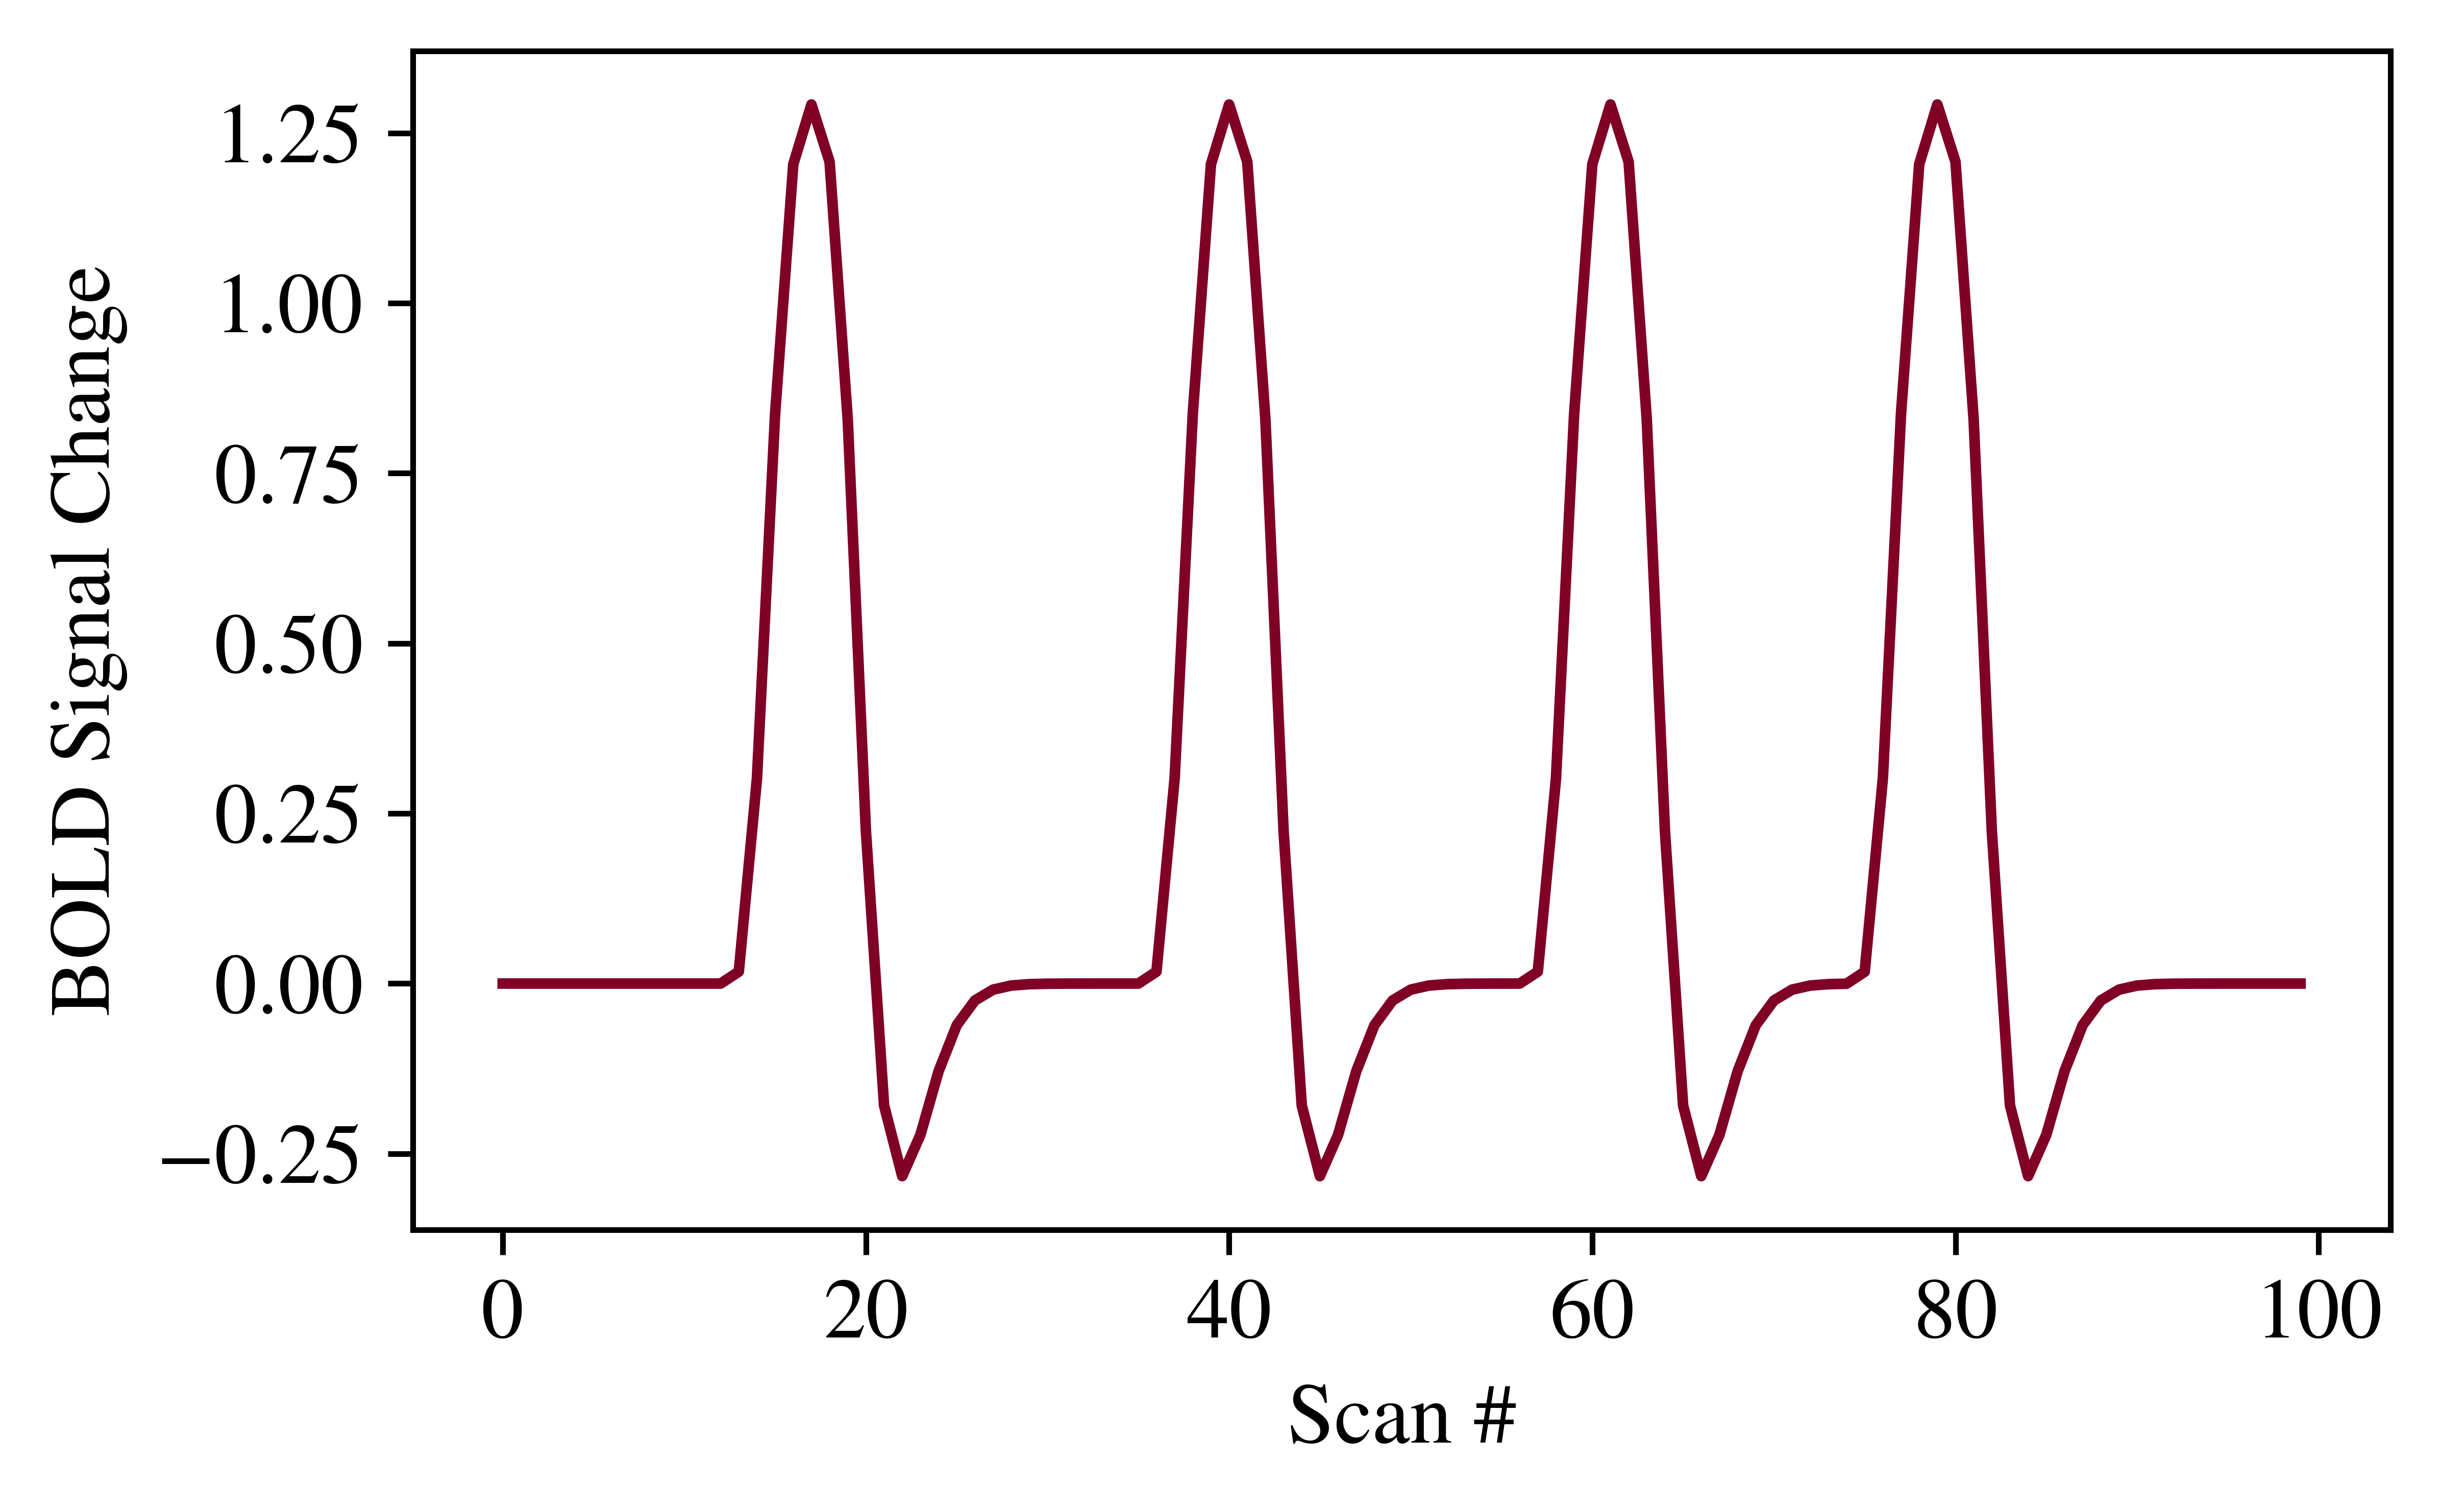
\includegraphics[width=0.89\textwidth]{images/gloverHRF.png}
\caption{Glover Hemodynamic Response Function}
\end{figure}
\end{frame}

\subsection{Previus Works}

%%%% 5
\begin{frame}{Previous Works}
\begin{itemize}
\item Identification of brain regions involved in language processing, memory, and 
decision-making \cite{gaillard2003developmental,golby2005memory,heekeren2003fmri}.
\item Identification of brain regions that are activated in response to specific 
stimuli or task \cite{orchard2003simultaneous, deneux2006using, ardekani1999activation}.
\item Methods used include time-series analysis, statistical parametric mapping, 
multivariate pattern classification, Bayesian modeling, among others 
\cite{adrian2018complex, marchini2004comparing, mumford2012deconvolving, makni2008fully}.
\item \gls{ast} method is also used by several researchers 
\cite{tabelow2006analyzing, lindquist2010adaptive, strappini2017adaptive,almodovar2019fast}.
\end{itemize}

\end{frame}

\subsection{Objectives}

%%%% 6
\begin{frame}{Objectives}
\begin{itemize}
\item Perform Bayesian time-series analysis to obtain a posterior probability 
map of an \gls{fmri} image for a single-subject situation.
\item Develop an \gls{ast} method that inputs the probability posterior map 
and finds the possible activated voxels.
\item Study the proposed algorithm in different simulation frameworks. Study 
the results in terms of similarity, rate of false positives, and \gls{poa}.
\item Finally, apply the algorithm to a real dataset.
\end{itemize}
\end{frame}

\section{Methods}

\subsection{Bayesian Analysis}

%%%% 7
\begin{frame}{Time Series Model}
\begin{itemize}
\item Each voxel has a time series associated to it.
\item Let $\bm{y}_i$ be the response variable of the $i$th voxel, $\bm{X}$ 
be the design matrix of the study containing the expected \gls{bold} change and 
$\bm{\beta}_i$ be the coefficient that contains the stimulus, then:

$$ \bm{y}_i \sim N \left( \bm{X} \bm{\beta}_i , \bm{\Sigma} \right)$$

\item Note that $\bm{\Sigma}$ can have any structure, however, if we 
let $\bm{\Sigma} = \sigma^2 \bm{I}$, the independent model is obtained:

$$ \bm{y}_i|\bm{\beta}_i, \sigma, \bm{X} \sim N \left( \bm{X} \bm{\beta}_i,\sigma^2\bm{I} \right) $$
\end{itemize}
\end{frame}

%%%% 8
\begin{frame}{Bayesian Approach}
\begin{itemize}
\item Using a noninformative prior distribution:

$$\pi \left( \bm{\beta}_i, \sigma \right) \propto \frac{1}{\sigma^{2}}$$

\item Using the Bayes' Rule and the ordinary least squares solution to a linear problem 
$\bm{\hat{\beta}}_i = \left( \bm{X}^T\bm{X} \right)^{-1}\bm{X}^T \bm{y}_i$, the 
conditional posterior of $\bm{\beta}_i$, given $\sigma$ is then:

$$\pi \left( \bm{\beta}_i|\sigma ,\bm{y}_i \right) \sim N\left( \bm{\hat{\beta}}_i, \left( \bm{X}^T\bm{X} \right)^{-1} \sigma^2 \right).$$
\end{itemize}
\end{frame}

%%%% 9
\begin{frame}{Posterior Probability Maps}
\begin{itemize}
\item Now, for each voxel, $i$, in the region of interest of our study, 
calculate the posterior probability that the coefficient associated with 
the stimulus, $t$, is not zero, which is roughly estimated using: 

$$P(\bm{\beta}_{i,t} > 0 | \bm{y}_i, \bm{X}).$$

\item Let 
$\bm{\mathbb{P}} = \left\{ P(\bm{\beta}_{i,t} > 0 | \bm{y}_i, \bm{X}) \right\}_{i=[1,v]}$ 
represent a Posterior Probability Map, where $v$ is the number of voxels in 
the region of interest of an \gls{fmri} experiment.
\end{itemize}
\end{frame}

%%%% 10
\begin{frame}{Posterior Probability Map}
\begin{figure}
\centering
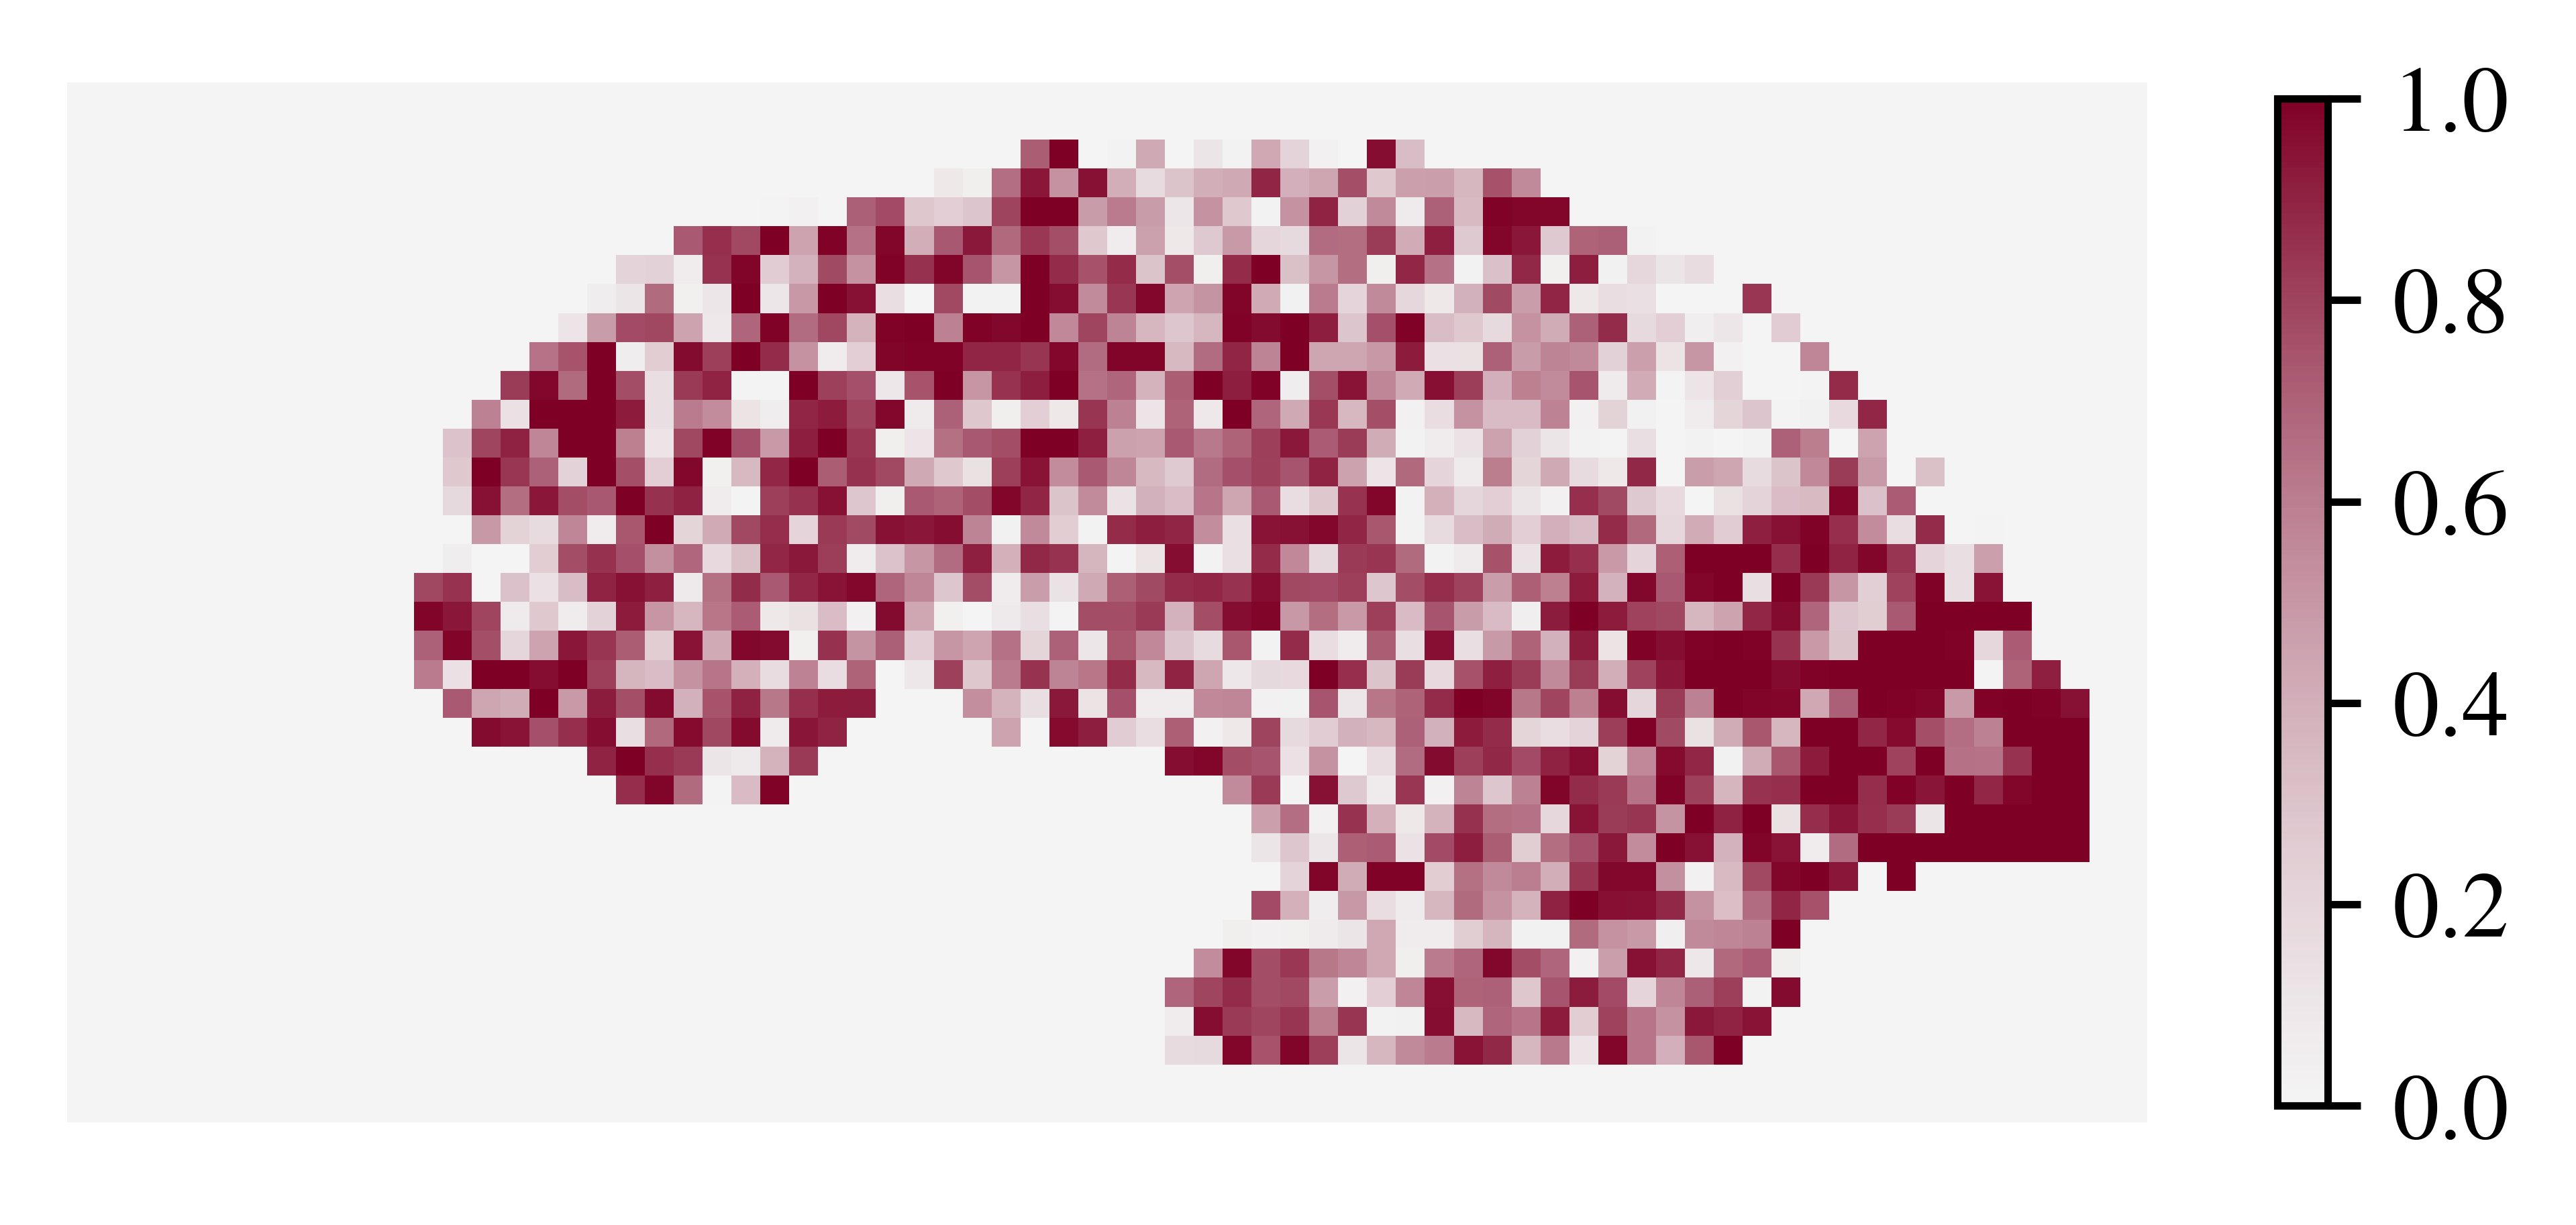
\includegraphics[width=0.9\textwidth]{Images/pMapEx.png}
\caption{Example of a Posterior Probability Map}
\end{figure}
\end{frame}

\subsection{bFAST Algorithm}

%%%% 11
\begin{frame}{Relevant Distributions}
\begin{itemize}
\item We will study $\bm{\mathbb{P}}$ as a \gls{tn} Distribution 
in the interval $[0,1]$.
\item $TN(0,1)$ is in the domain of maximal attraction of the limiting 
distribution $G$, a Gumbel distribution.
\begin{itemize}
\item Therefore, $TN^v(a_vx+b_v) \rightarrow G(x)$.
\item For $a_v = \left[ v \psi (b_v) \right]^{-1}$ and $b_v = \Psi^{-1}(1-1/v)$.
\item Where $\psi$ and $\Psi$ are the PDF and CDF of the $TN$, respectively.
\end{itemize}
\end{itemize}
\end{frame}

%%%% 12
\begin{frame}{Gaussian Kernel Smoothing}
\begin{itemize}
\item Convolution of the image with:
\begin{itemize}
\item Gaussian function in 2D: 
$G(x,y) = \frac{1}{2\pi\sigma_{s}^2} \exp \left( -\frac{x^2+y^2}{2\sigma_{s}^2} \right)$.
\item This can be extended to 3D.
\end{itemize}
\end{itemize}
\begin{figure}
\centering
\includegraphics[width=0.8\textwidth]{images/pMapExSmoothing.png}
\caption{Example of the Smoothing Process in Posterior Probability Map}
\end{figure}
\end{frame}

%%%% 13
\begin{frame}{\acrfull{ji}}
\begin{itemize}
\item Used to calculate image similarity:
\begin{itemize}
\item $ J(\bm{A},\bm{B}) = \frac{|\bm{A} \cap \bm{B}|}{|\bm{A} \cup \bm{B}|} $
\end{itemize}
\end{itemize}
\begin{figure}
\centering
\includegraphics[width=0.7\textwidth]{images/jiEx.png}
\caption{Example of Similarity Measurement Using \acrshort{ji}}
\end{figure}
\end{frame}

%%%% 14
\begin{frame}{bFAST Algorithm}
\begin{itemize}
\item Initialization
\begin{itemize}
\item $\bm{\mathbb{P}^{(0)}} = \bm{\mathbb{P}}$
\item $\zeta_i \equiv 0 \forall i$, where $\zeta_i$ is 1 when voxel $i$ is activated and 0 if not.
\item $\zeta_i^{(0)} \equiv \zeta_i$
\item $v_0 = v$, where $v_k$ is the number of voxels for which $\zeta_i^{(k)} = 0$.
\end{itemize}
\end{itemize}
\end{frame}

%%%% 15
\begin{frame}{bFAST Algorithm}
\begin{itemize}
\item For $k=1,2,\dots,$ iterate as follows:
\begin{itemize}
\item \textit{Smoothing}. Smooth $\bm{\mathbb{P}^{(k-1)}}$ using a Gaussian Kernel to obtain $\bm{\mathbb{P}^{(k)}}$. Let $\sigma_s = 0.65 + 100(k - 1)$.
\item \textit{Thresholding.} This consists of three steps:
\begin{itemize}
\item Estimate $\bm{\mathbb{P}^{(k-1)}}$ as a \gls{tn}.
\item Calculate $a_v$ and $b_v$.
\item Calculate the probability threshold, $\eta=a_v\iota_{0.01}+b_v$, with $\iota_{0.01}$ be the upper-tail $0.01$-value of the standard Gumbel Distribution.
\end{itemize}
\item \textit{Activation}: Set $\zeta_i^{(k)} = 1$ if $\zeta_i^{(k-1)} = 0$ and the value of the $i$th voxel of $\bm{\mathbb{P}^{(k)}}$ is greater than $\eta$. Calculate $v_k=\sum_{i=1}^v\zeta_i^{(k)}$.
\end{itemize}
\end{itemize}
\end{frame}

%%%% 16
\begin{frame}{bFAST Algorithm}
\begin{itemize}
\item Termination
\begin{itemize}
\item Declare no activation and terminate if $\bm{\zeta}^{(1)} \equiv 0$.
\item If $J(\bm{\zeta}^{(k)},\bm{\zeta}^{(k-1)}) \geq J(\bm{\zeta}^{(k+1)},\bm{\zeta}^{(k)})$, the algorithm terminates and the final activation map is $\bm{\zeta}^{(k)}$.
\item The maximum number of iterations is default to $k=10$.
\end{itemize}
\end{itemize}
\end{frame}

\section{Simulations}

\subsection{True Maps}

%%%% 17
\begin{frame}{True Maps Summary}
\begin{table}
\centering
\caption{Details of True Maps Considered. In both maps, dark voxels are active and light voxels are inactive.}
\begin{tabular}{x{2.1cm}x{3.5cm}x{3.5cm}}
\hline
\textbf{Name} & \textbf{2D} & \textbf{3D} \\ \hline
Dimensions & $200 \times 200$ & $40 \times 40 \times 25$ \\
Voxels & 40000 & 40000 \\ 
\gls{poa} & 19.9375 & 3.9525 \\
Map & 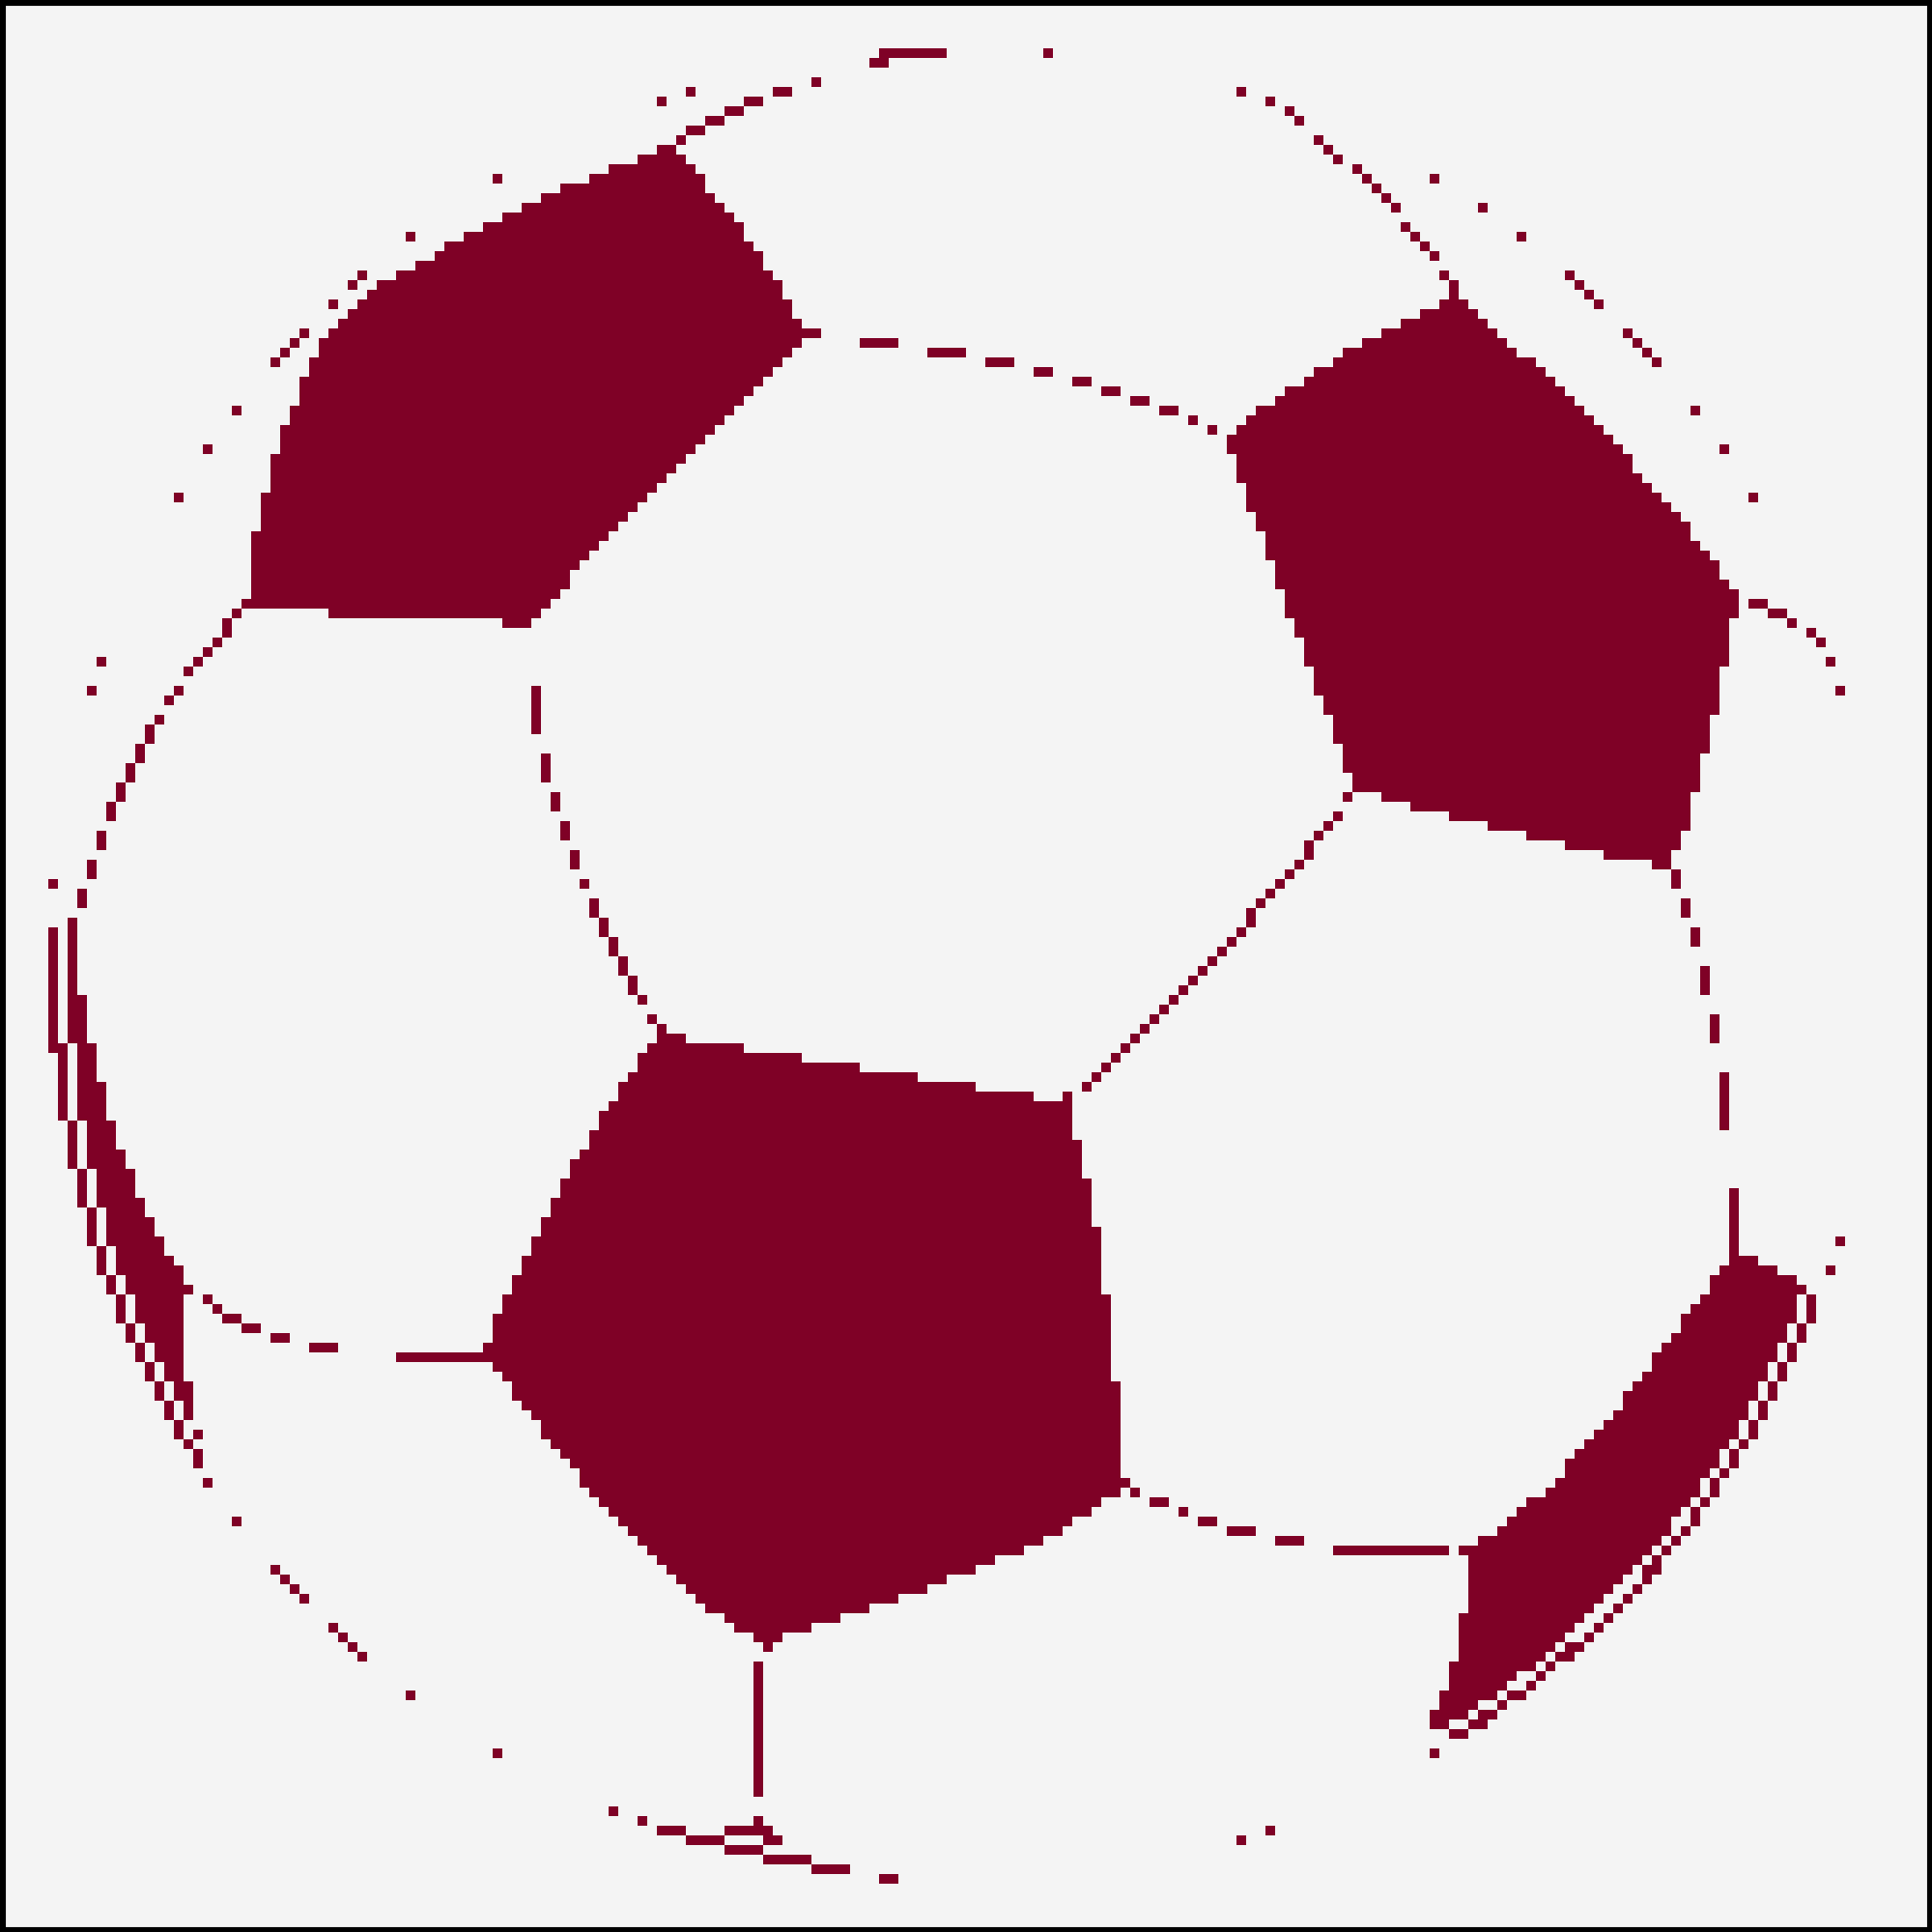
\includegraphics[width=0.28\textwidth]{images/aMap2D.png} & 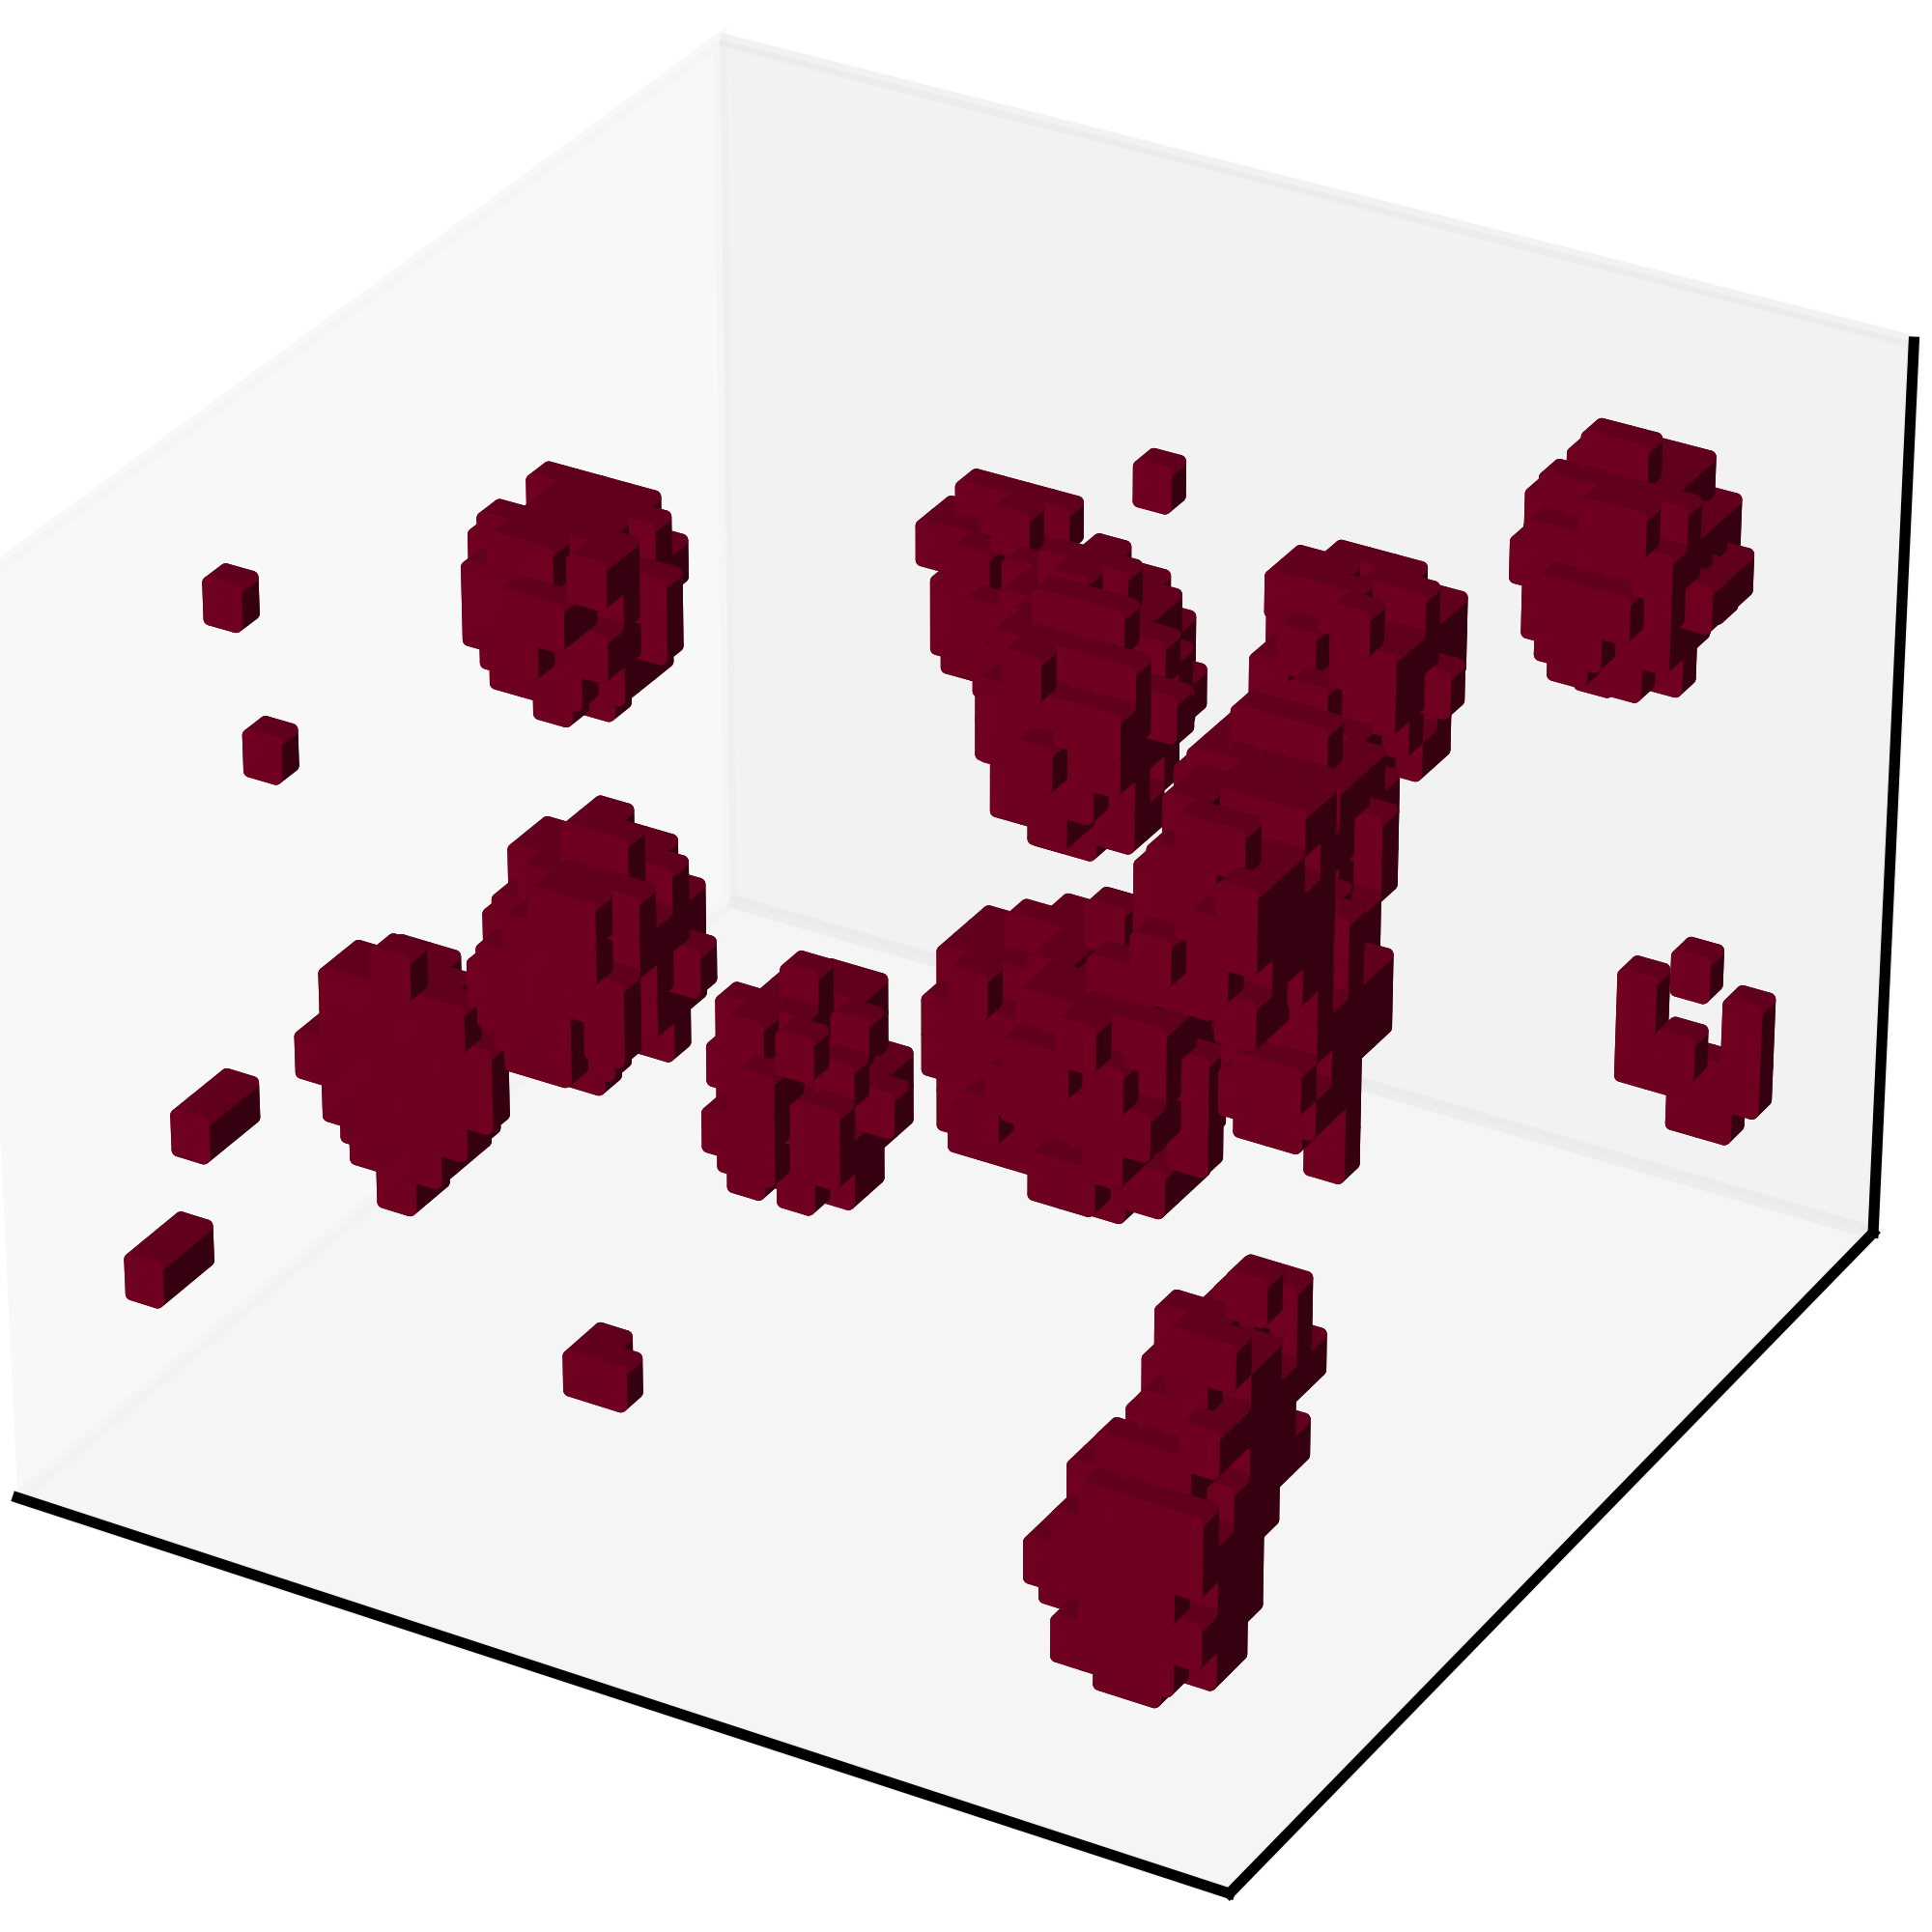
\includegraphics[width=0.28\textwidth]{images/aMap3D.png} \\ \hline
\end{tabular}
\end{table}
\end{frame}

%%%% 18
\begin{frame}{3D Map Creation}
\begin{itemize}
\item Step 1. Create a random $40 \times 40$ grid of numbers between 0 and 1. 
The ones that are greater than 0.99 take a value of 1, the rest are 0.
\item Step 2. For each of those ones, select a random integer between 1 and 25 
to be the depth of the cluster in the 3D grid.
\item Step 3. At each of the cluster centers, generate a ball of radius 5. 
For each voxel inside that ball, randomly mark as active only the $67\%$ of them.
\item Step 4. Identify inactive voxels in each cluster that are surrounded by at 
least 4 active voxels. If so, mark it as active.
\end{itemize}
\end{frame}

\subsection{Design Matrix}

%%%% 19
\begin{frame}{Design Matrix}
\begin{itemize}
\item $\bm{X}$ will consist of 2 columns and one row per scan.
\item The second column corresponds to the constant regressor.
\item The first column contains the Glover Hemodynamic Response Function
 given the following event description:

\begin{table}
\centering
\caption{Event Description of Simulated \gls{fmri} Experiment}
\begin{tabular}{cc}
\hline
\textbf{Parameter} & \textbf{Value} \\ \hline
Number of Scans & 100 \\
Time Between Scans & 2 seconds \\
Number of Stimulus & 4 \\
Duration of Each Stimulus & 10 seconds \\
Time Between Stimulus & 18 - 25 seconds \\ \hline
\end{tabular}
\end{table}
\end{itemize}
\end{frame}

\subsection{BOLD}

%%%% 20
\begin{frame}{\acrshort{bold}}
\begin{itemize}
\item \gls{bold} response without noise is computed depending on the voxel 
activation status, $\zeta_i$, on the true map. See Table \ref{tab:parSelA}.

\begin{table}
\centering
\caption{Parameter Selection Based on Activation Status}
\begin{tabular}{cc}
\hline
\textbf{Activation Status} & \textbf{Parameter Values} \\ \hline
$\zeta_i=0$ & $\bm{\beta^*}_i = (0,100)^T$ \\
$\zeta_i=1$ & $\bm{\beta^*}_i = (75,100)^T$ \\ \hline
\end{tabular}
\label{tab:parSelA}
\end{table}

\item BOLD response, $\bm{y}_i$, for each voxel $i$ depends on the \gls{bold} 
response without noise, $\bm{X}\bm{\beta^*}_i$, and the noise generated 
using an $ARMA$ Model, $\bm{\epsilon}$:
$$
\bm{y}_i = \bm{X}\bm{\beta^*}_i + \bm{\epsilon}.
$$
\end{itemize}
\end{frame}

\subsection{Noise}

%%%% 21
\begin{frame}{Noise with ARMA}
\begin{itemize}
\item The noise ($\bm{\epsilon}$) is a vector of mean $\mu = 0$ and variance 
$\sigma^2=25^2$ with a baseline structure equivalent to: 
$$ARMA_{\bm{\epsilon}}\left( \{p_1,p_2,\dots\},\{q_1,q_2,\dots\} \right).$$

\item $p = \left| \{p_1,p_2,\dots\} \right|$ and $q= \left| \{q_1,q_2,\dots\} \right|$ are 
related to the order of the corresponding $ARMA$ model, where $p_a$ and $q_b$ represent the 
coefficients of such models.

\item $p,q \in [0,1,2,3]$ were chosen to study the model under 
different noise scenarios. The values of $p_a$, and $q_b$ were chosen arbitrarily 
as parameters. See Table \ref{tab:parSelE}.

\end{itemize}
\end{frame}

%%%% 22
\begin{frame}{Noise with ARMA}
\begin{table}
\centering
\caption{Parameter Selection Related to $\bm{\epsilon}$}
\resizebox{\columnwidth}{!}{
\begin{tabular}{cccccc}
&&\multicolumn{4}{c}{$p$} \\
&\hspace{6pt} \arrvline&0&1&2&3 \\ \cline{2-6}
\multirow{4}{*}{$q$}&0 \arrvline & $\{\},\{\}$&$\{\frac{1}{2}\},\{\}$&$\{\frac{1}{2},\frac{3}{10}\},\{\}$&$\{\frac{1}{2},\frac{3}{10},\frac{1}{10}\},\{\}$ \\
&1 \arrvline & $\{\},\{\frac{1}{2}\}$&$\{\frac{1}{2}\},\{\frac{1}{2}\}$&$\{\frac{1}{2},\frac{3}{10}\},\{\frac{1}{2}\}$&$\{\frac{1}{2},\frac{3}{10},\frac{1}{10}\},\{\frac{1}{2}\}$ \\
&2 \arrvline & $\{\},\{\frac{1}{2},\frac{3}{10}\}$&$\{\frac{1}{2}\},\{\frac{1}{2},\frac{3}{10}\}$&$\{\frac{1}{2},\frac{3}{10}\},\{\frac{1}{2},\frac{3}{10}\}$&$\{\frac{1}{2},\frac{3}{10},\frac{1}{10}\},\{\frac{1}{2},\frac{3}{10}\}$ \\
&3 \arrvline & $\{\},\{\frac{1}{2},\frac{3}{10},\frac{1}{10}\}$&$\{\frac{1}{2}\},\{\frac{1}{2},\frac{3}{10},\frac{1}{10}\}$&$\{\frac{1}{2},\frac{3}{10}\},\{\frac{1}{2},\frac{3}{10},\frac{1}{10}\}$&$\{\frac{1}{2},\frac{3}{10},\frac{1}{10}\},\{\frac{1}{2},\frac{3}{10},\frac{1}{10}\}$
\end{tabular}
}
\label{tab:parSelE}
\end{table}
\end{frame}

%%%% 23
\begin{frame}{\acrshort{snr} and \acrshort{cnr}}
\begin{itemize}
\item \acrfull{snr} represents how strong the signal is with respect to the noise.
\begin{itemize}
\item Generally, the \gls{snr} value of an \gls{fmri} experiment is around 4.
\end{itemize}
\item \acrfull{cnr} represents how significant is the \gls{bold} change in 
activation regions with respect to the noise.
\begin{itemize}
\item Generally, the \gls{cnr} value of an \gls{fmri} experiment is around 3.
\end{itemize}
\end{itemize}
\end{frame}

\section{Results}

\subsection{Noise}

%%%% 24
\begin{frame}{Noise in Simulations}
\begin{figure}
\centering
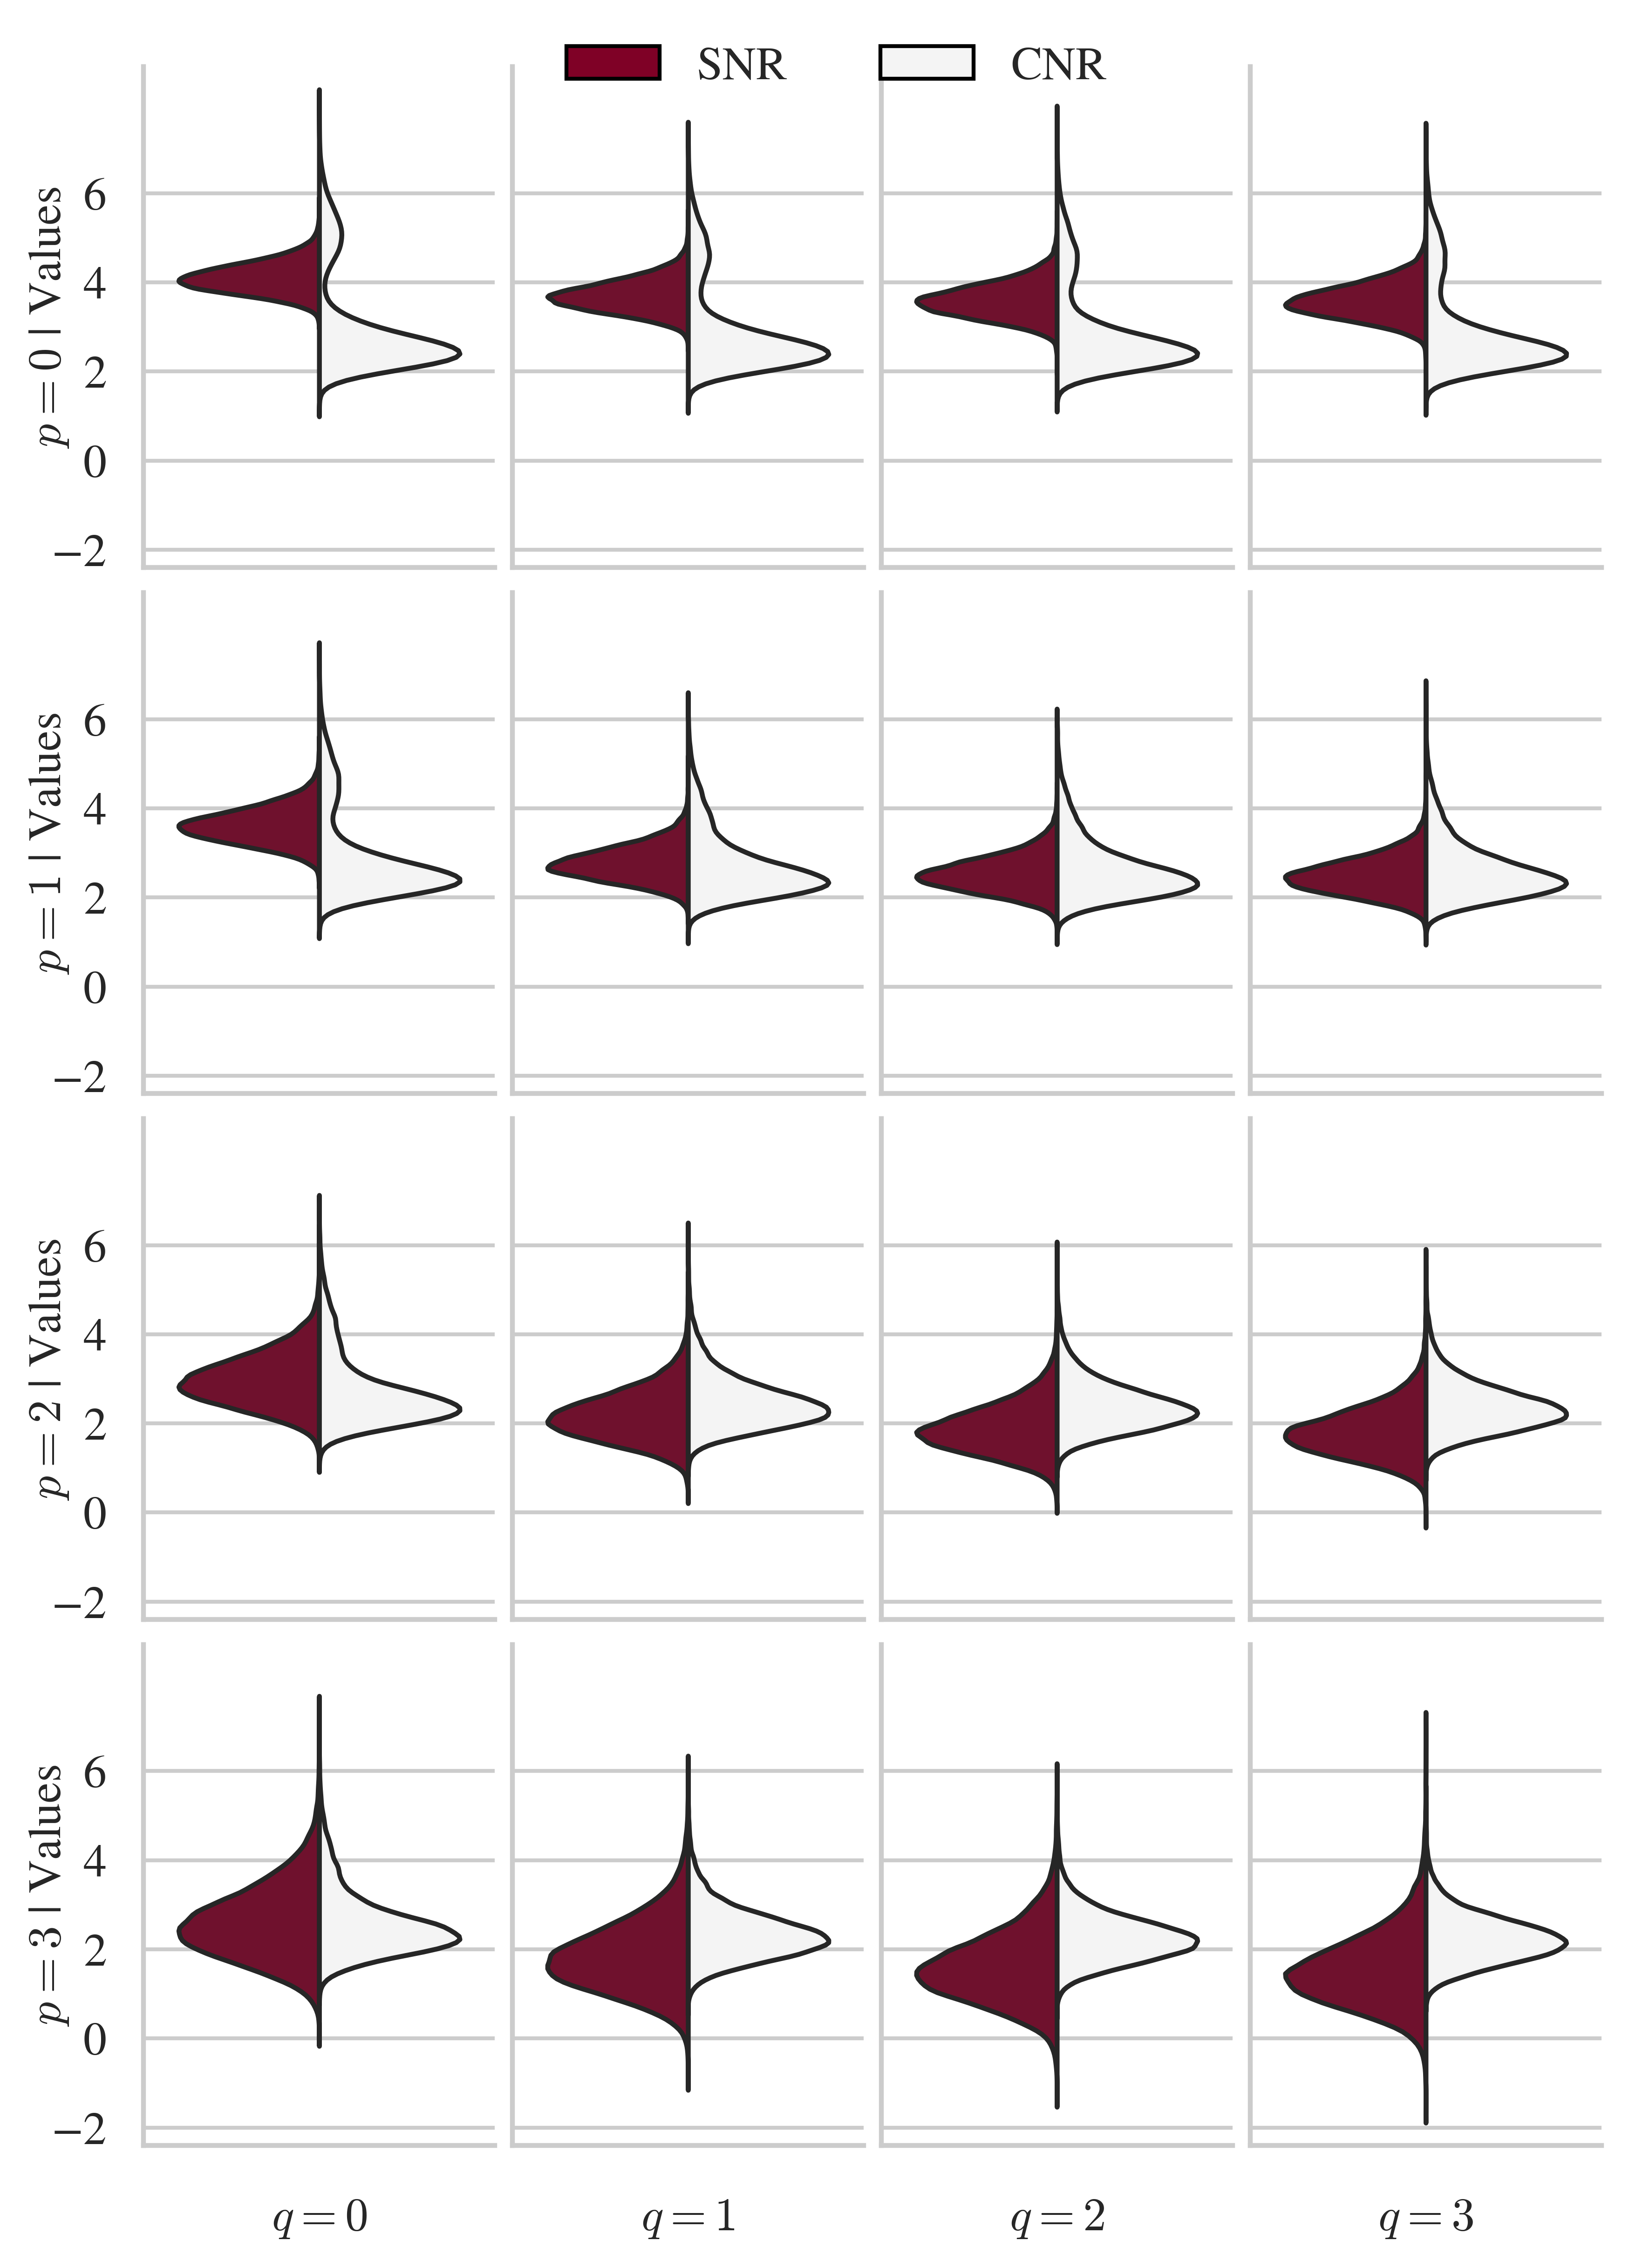
\includegraphics[width=0.4\textwidth]{Images/cnrsnr2D.png}
\caption{Numerical Distribution of the Voxel-Wise \gls{snr} and \gls{cnr} Values of 2D Map}
\end{figure}
\end{frame}

%%%% 25
\begin{frame}{Noise in Simulations}
\begin{figure}
\centering
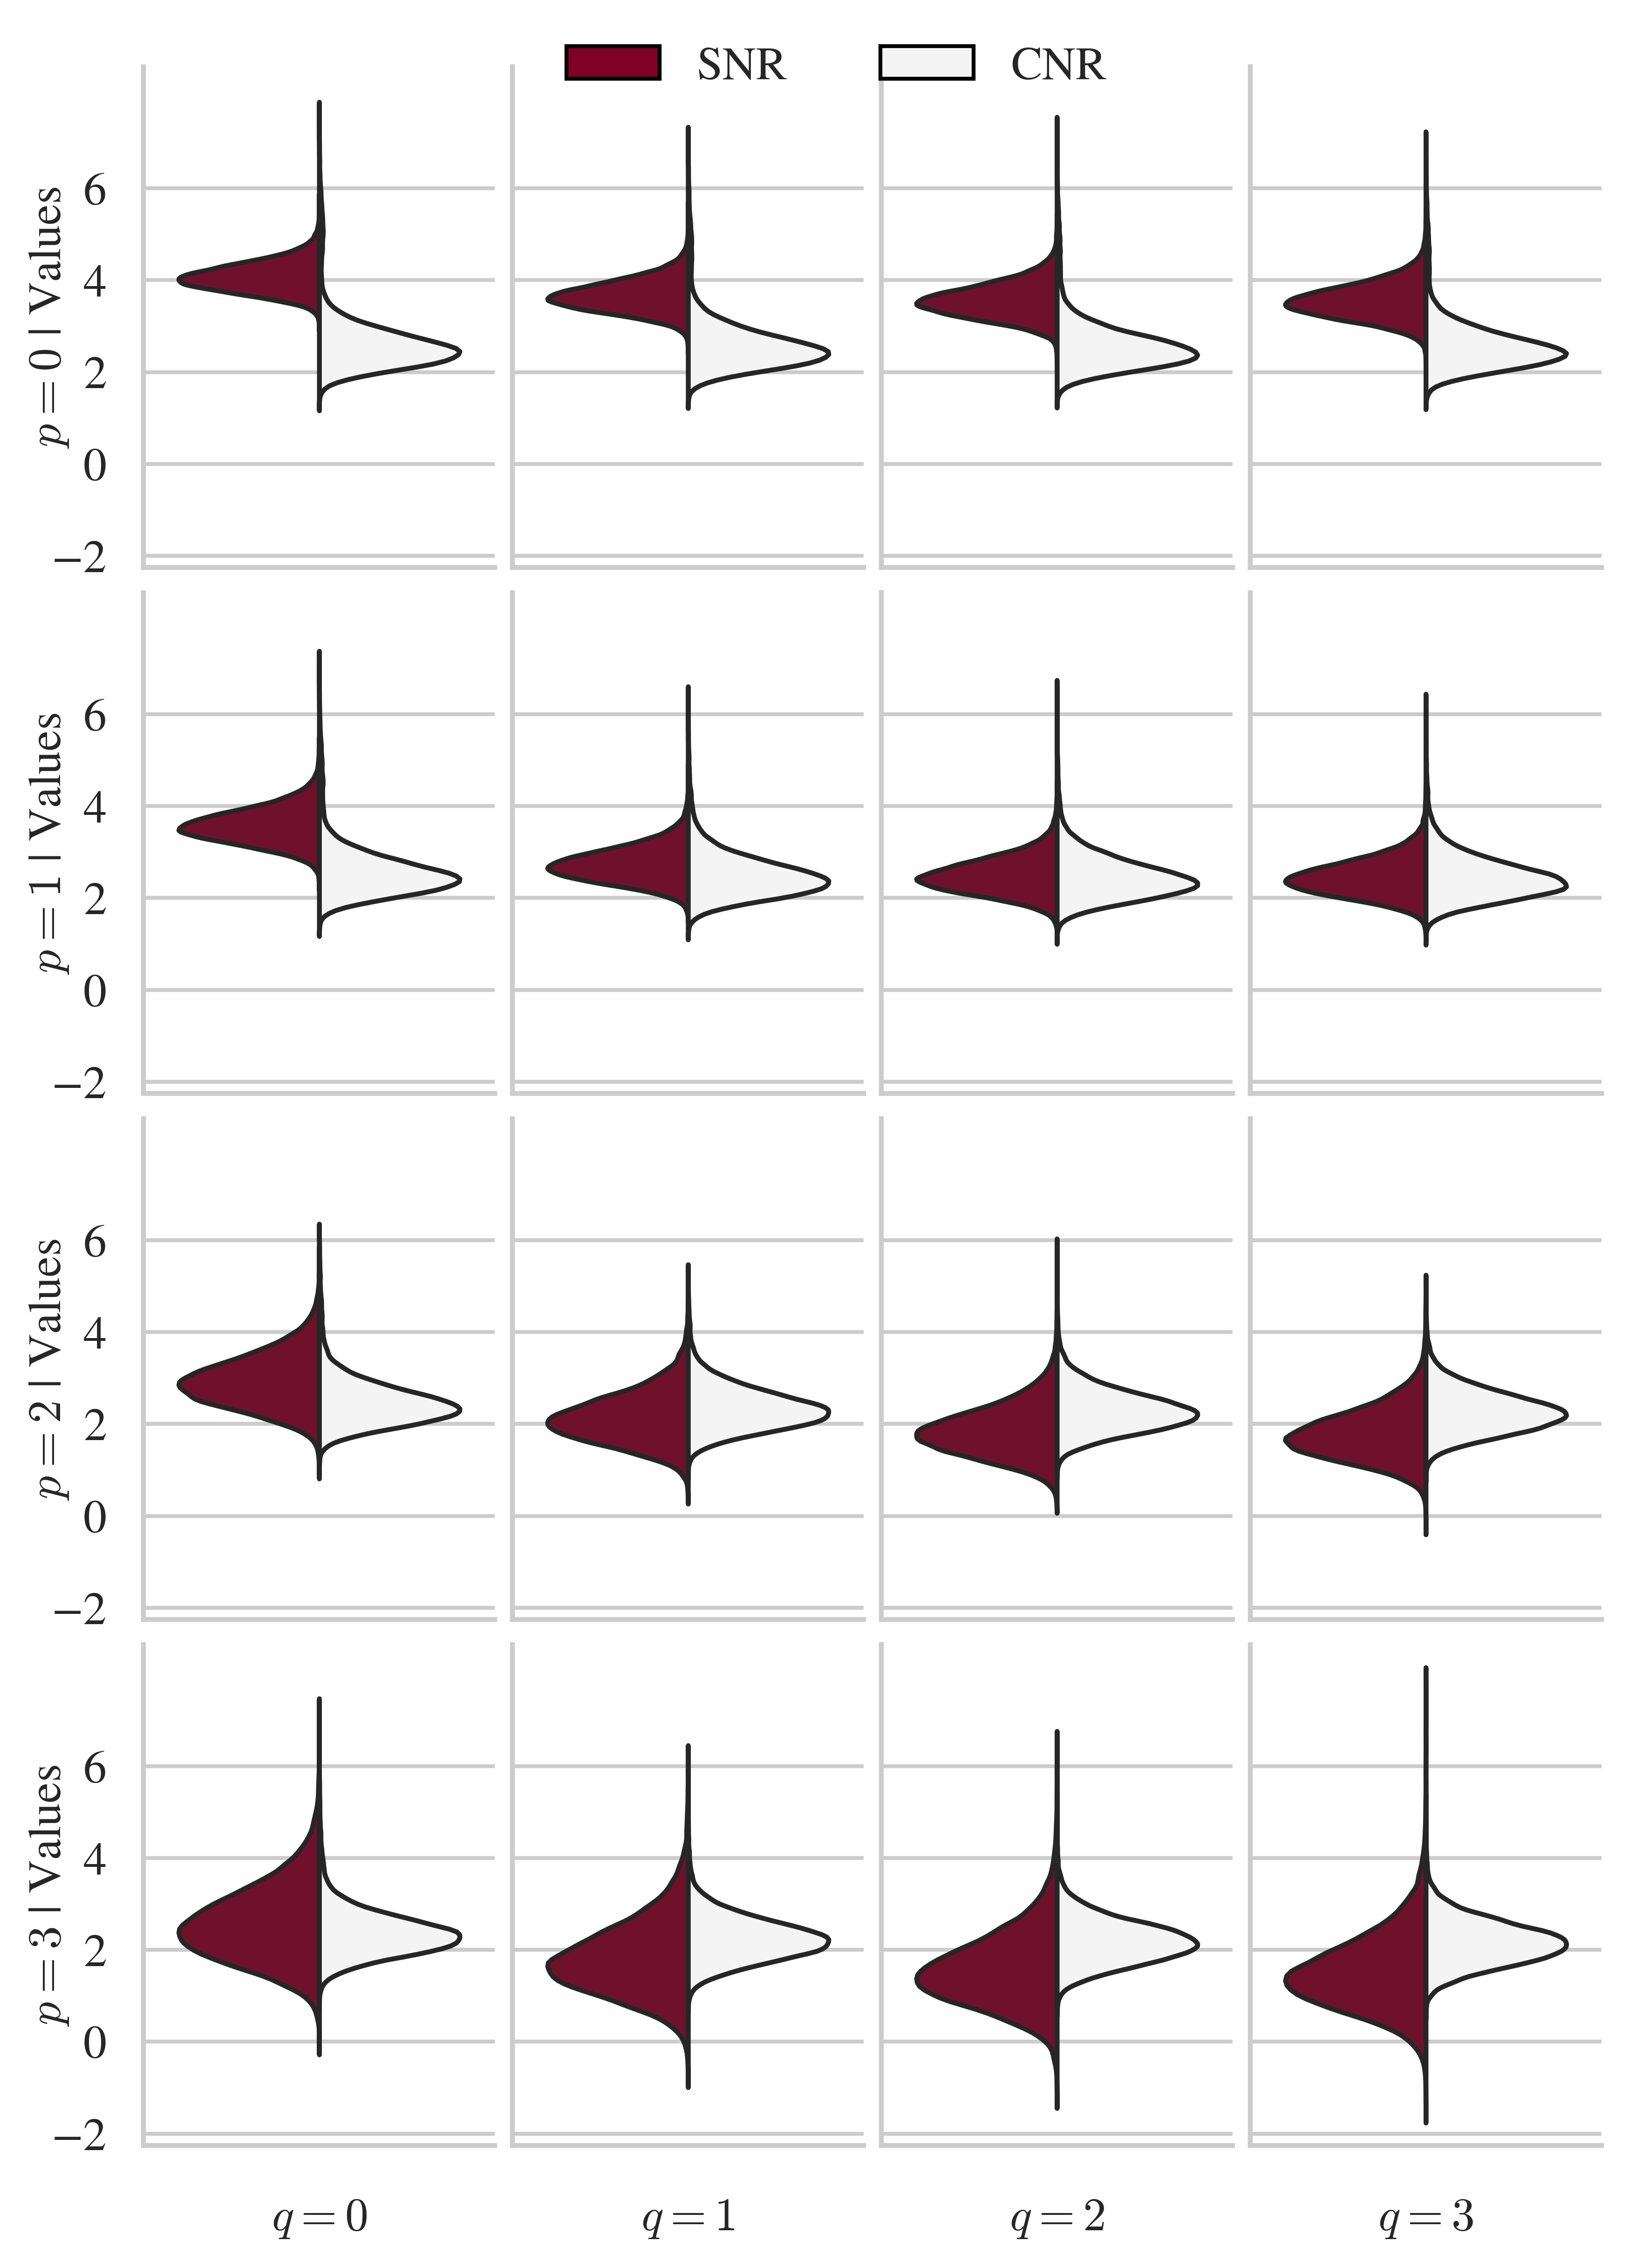
\includegraphics[width=0.4\textwidth]{Images/cnrsnr3D.png}
\caption{Numerical Distribution of the Voxel-Wise \gls{snr} and \gls{cnr} Values of 3D Map}
\end{figure}
\end{frame}

%%%% 26
\begin{frame}{Noise in Simulations}
\begin{columns}
\column{0.49\linewidth}
\begin{figure}
\centering
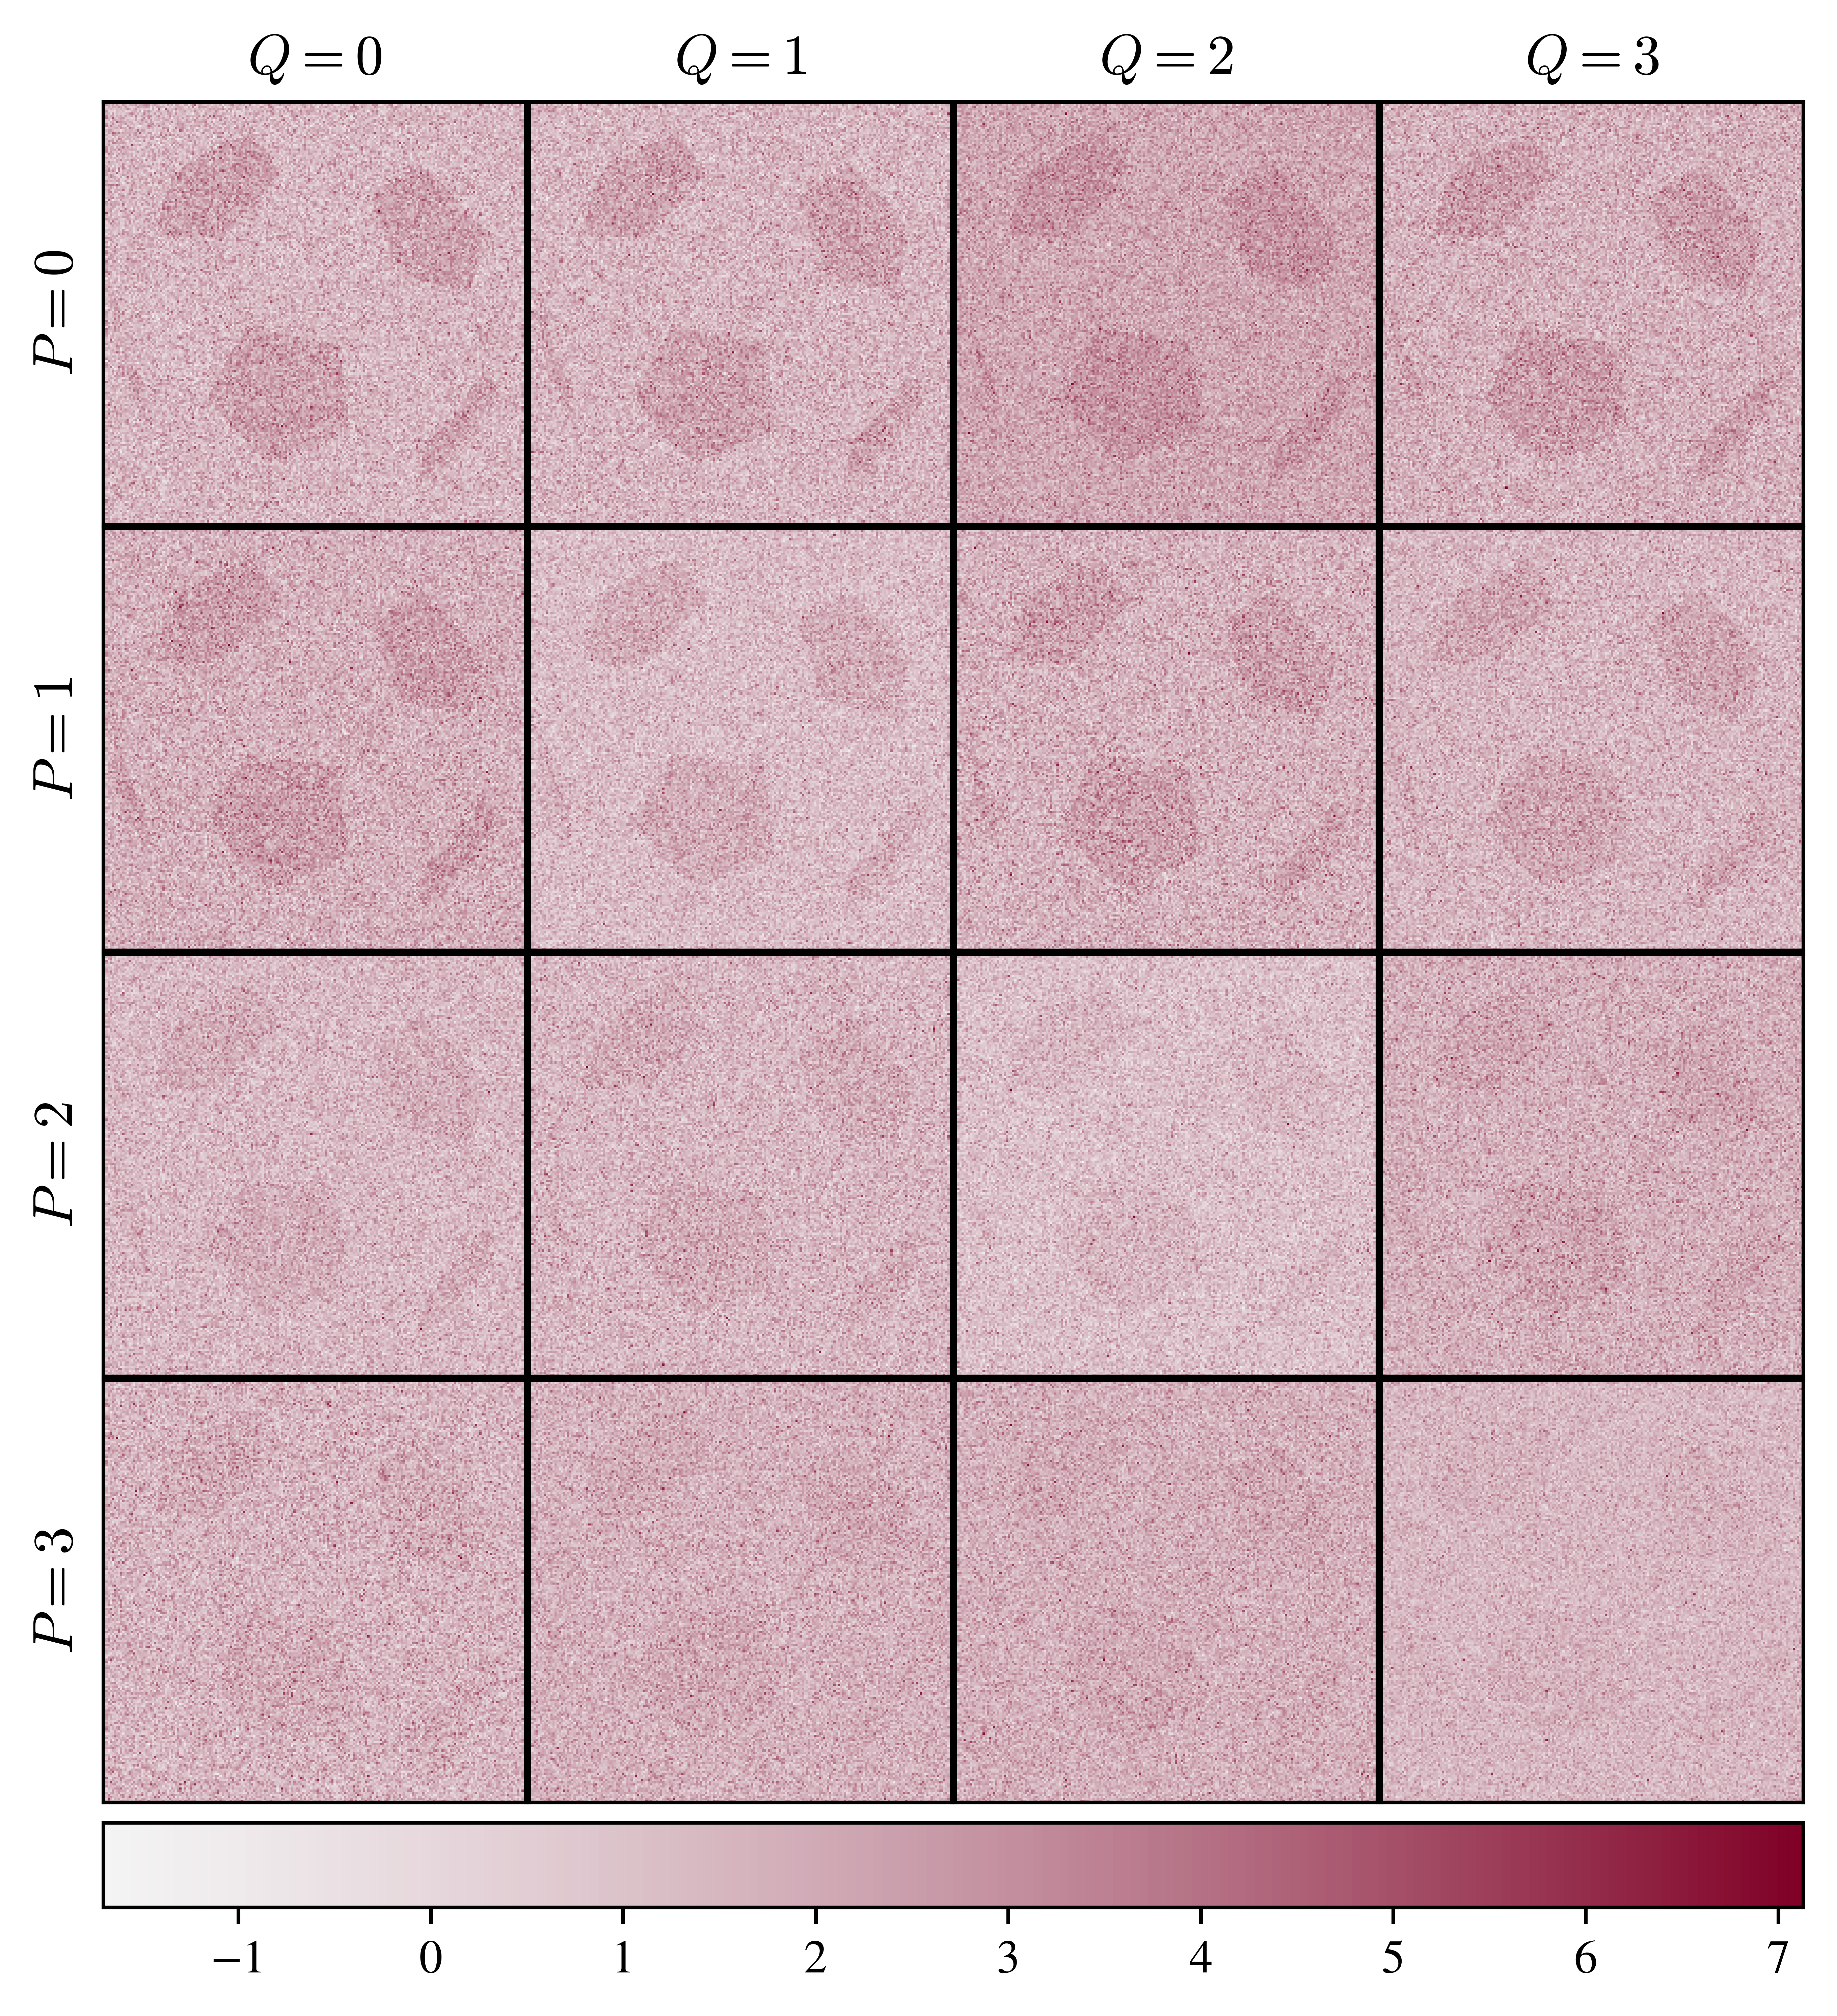
\includegraphics[width=0.9\textwidth]{Images/snr2D_Spatial.png}
\caption{Spatial Distribution of the \gls{snr} Values in 2D Map}
\end{figure}

\column{0.49\linewidth}
\begin{figure}
\centering
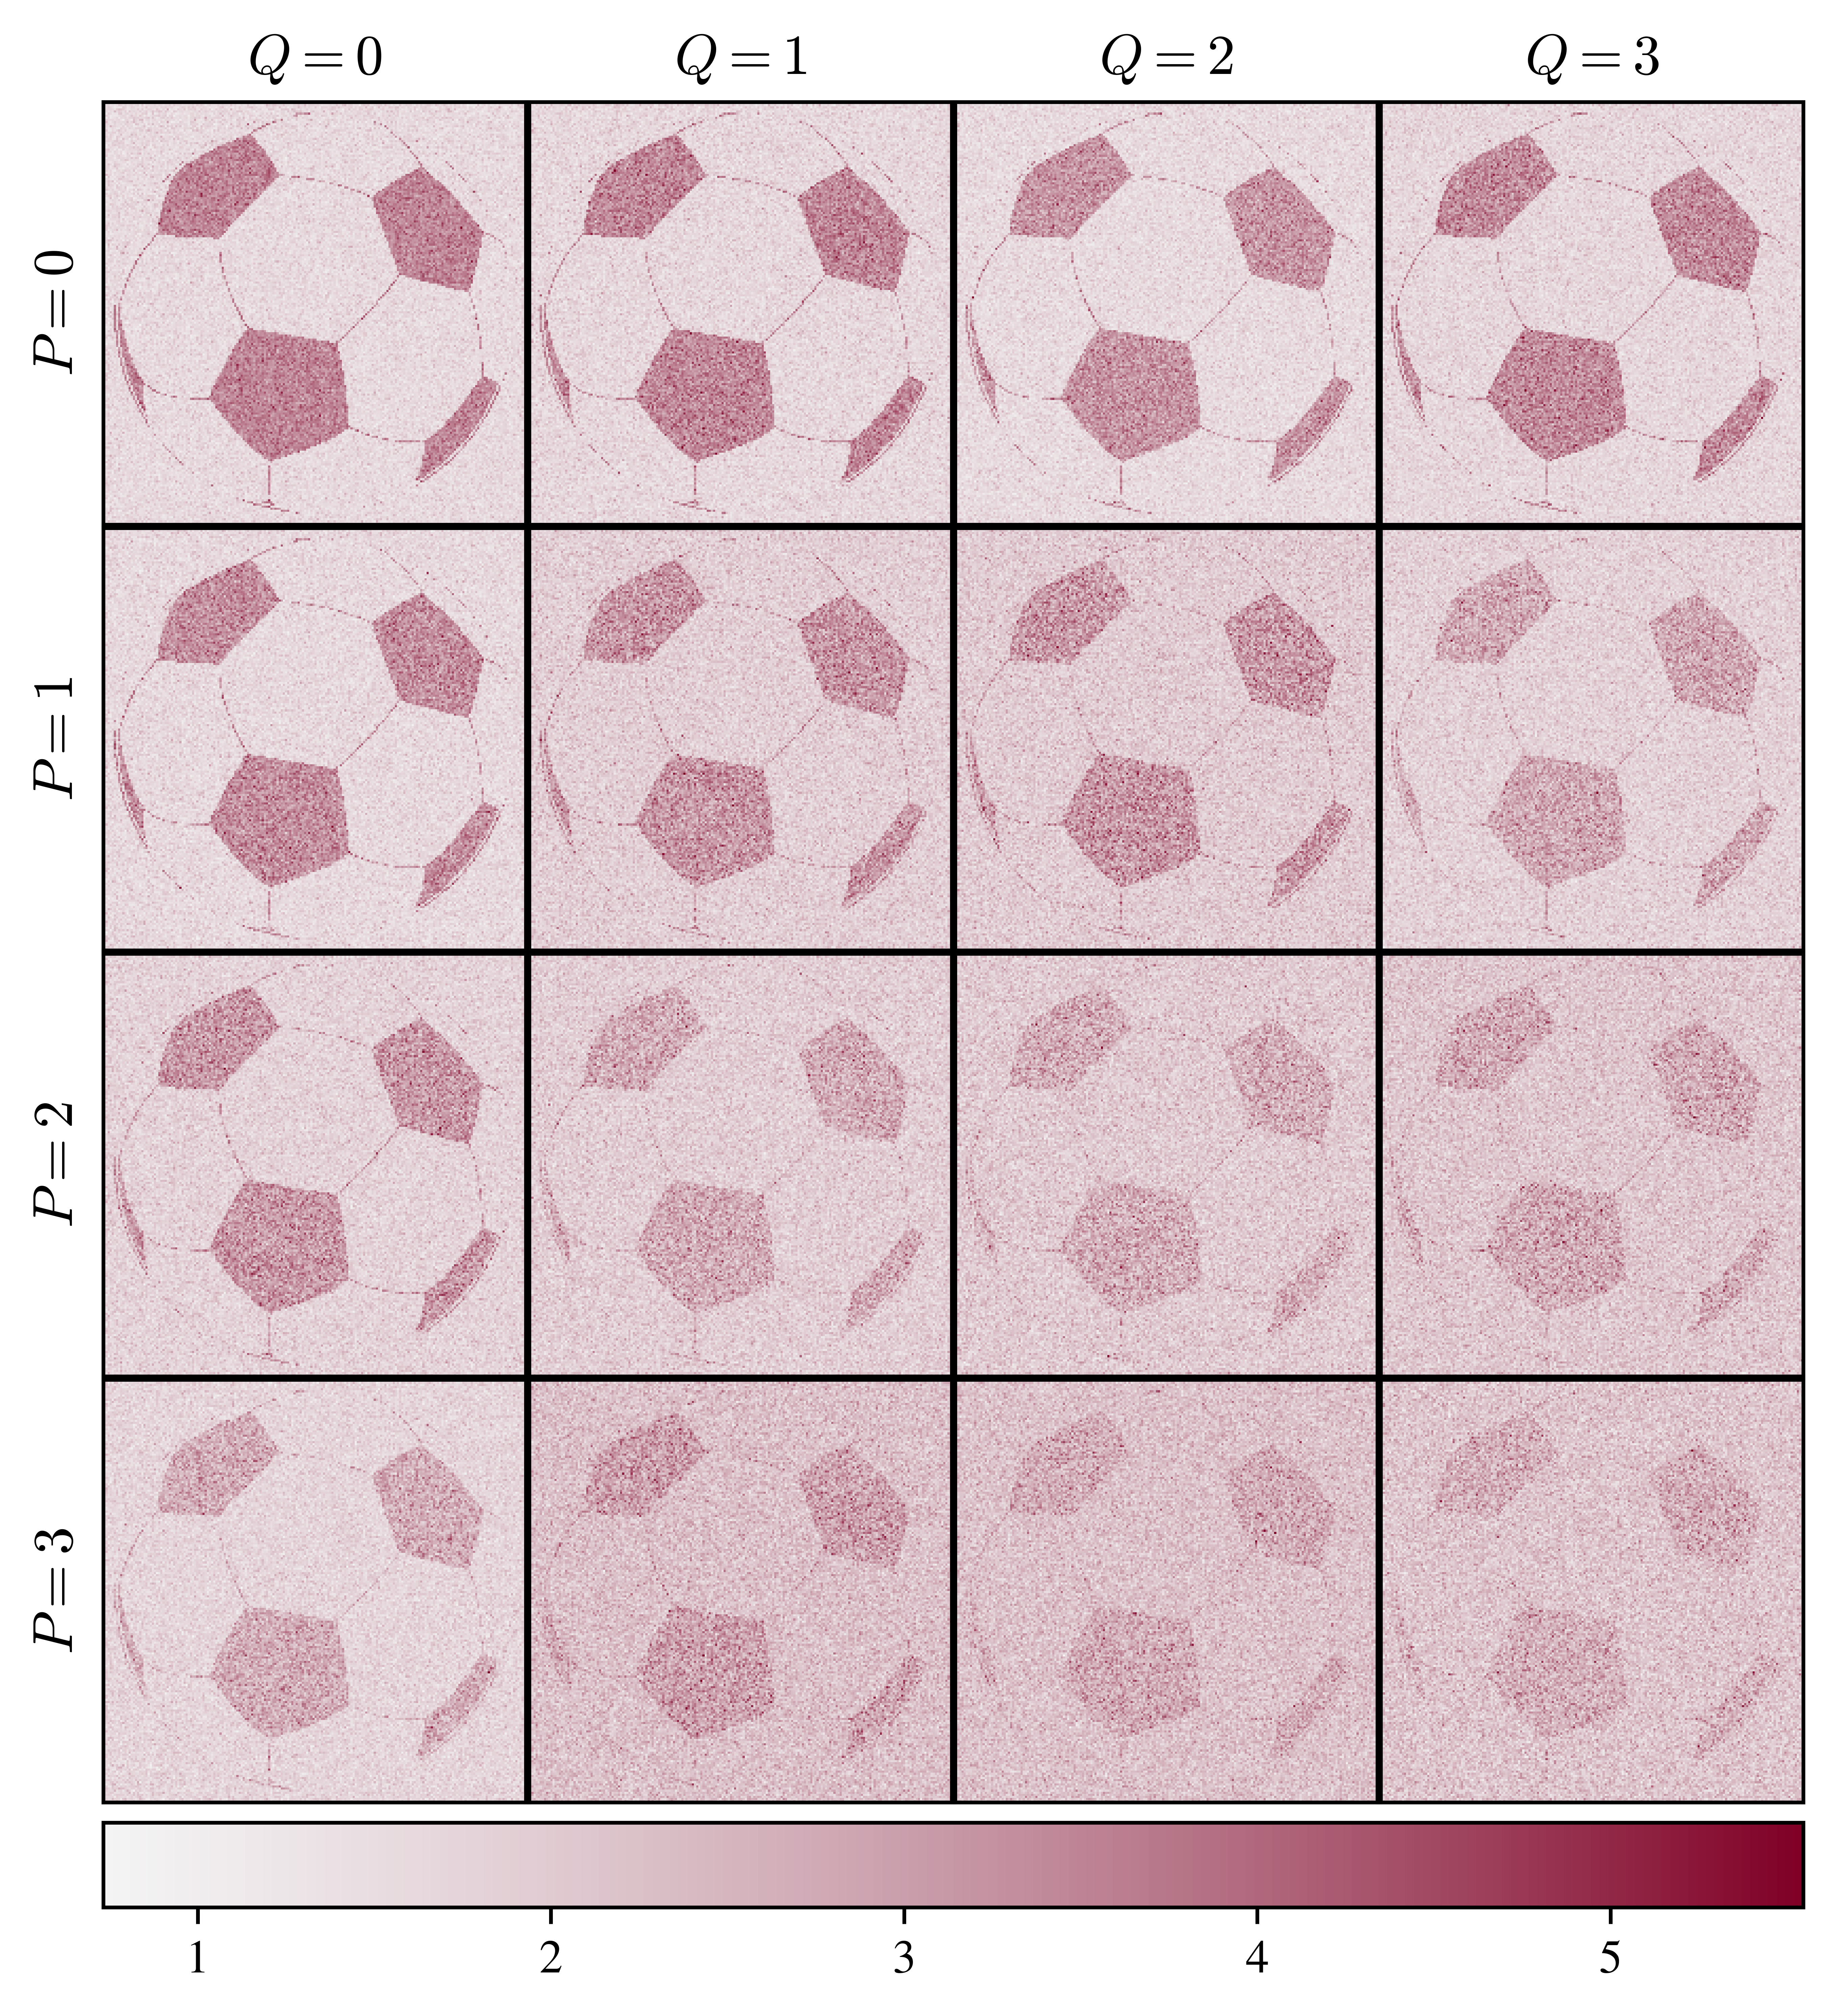
\includegraphics[width=0.9\textwidth]{Images/cnr2D_Spatial.png}
\caption{Spatial Distribution of the \gls{cnr} Values in 2D Map}
\end{figure}
\end{columns}
\end{frame}

\subsection{Iterations Example}

%%%% 27
\begin{frame}{Example of bFAST Iterations}
\begin{figure}
\centering
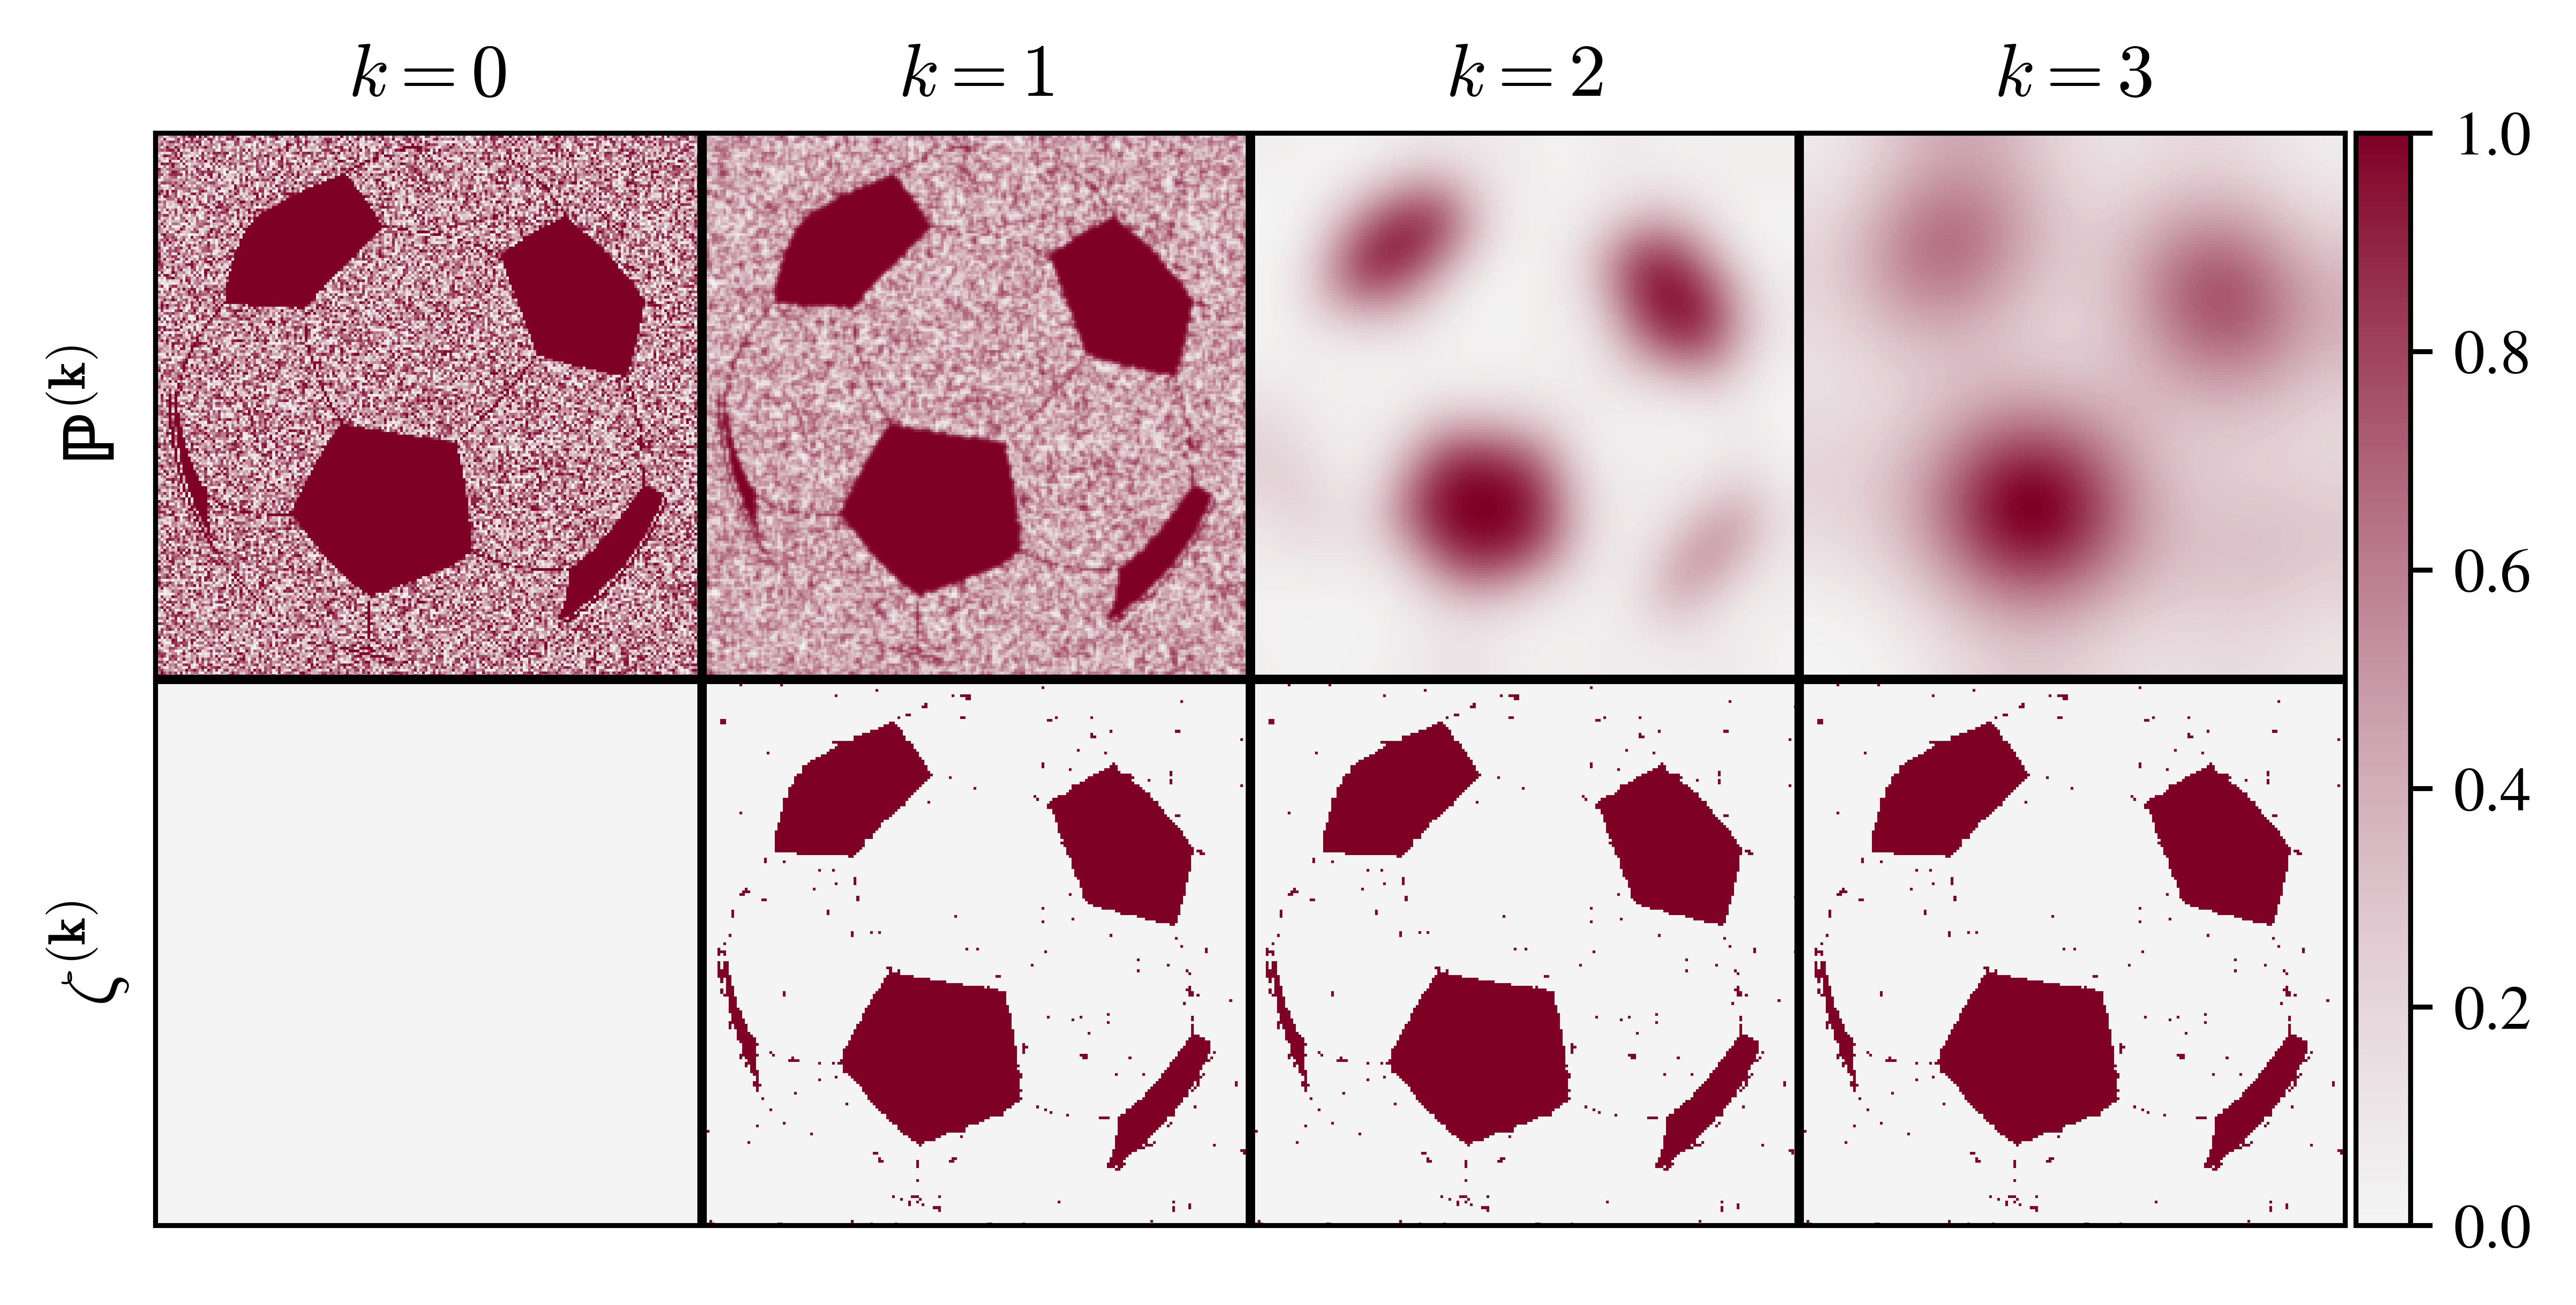
\includegraphics[width=0.65\textwidth]{Images/bfastEx2D.png}
\caption{Example in 2D Map for $p,q=0$}
\end{figure}
\end{frame}

%%%% 28
\begin{frame}{Example of bFAST Iterations}
\begin{figure}
\centering
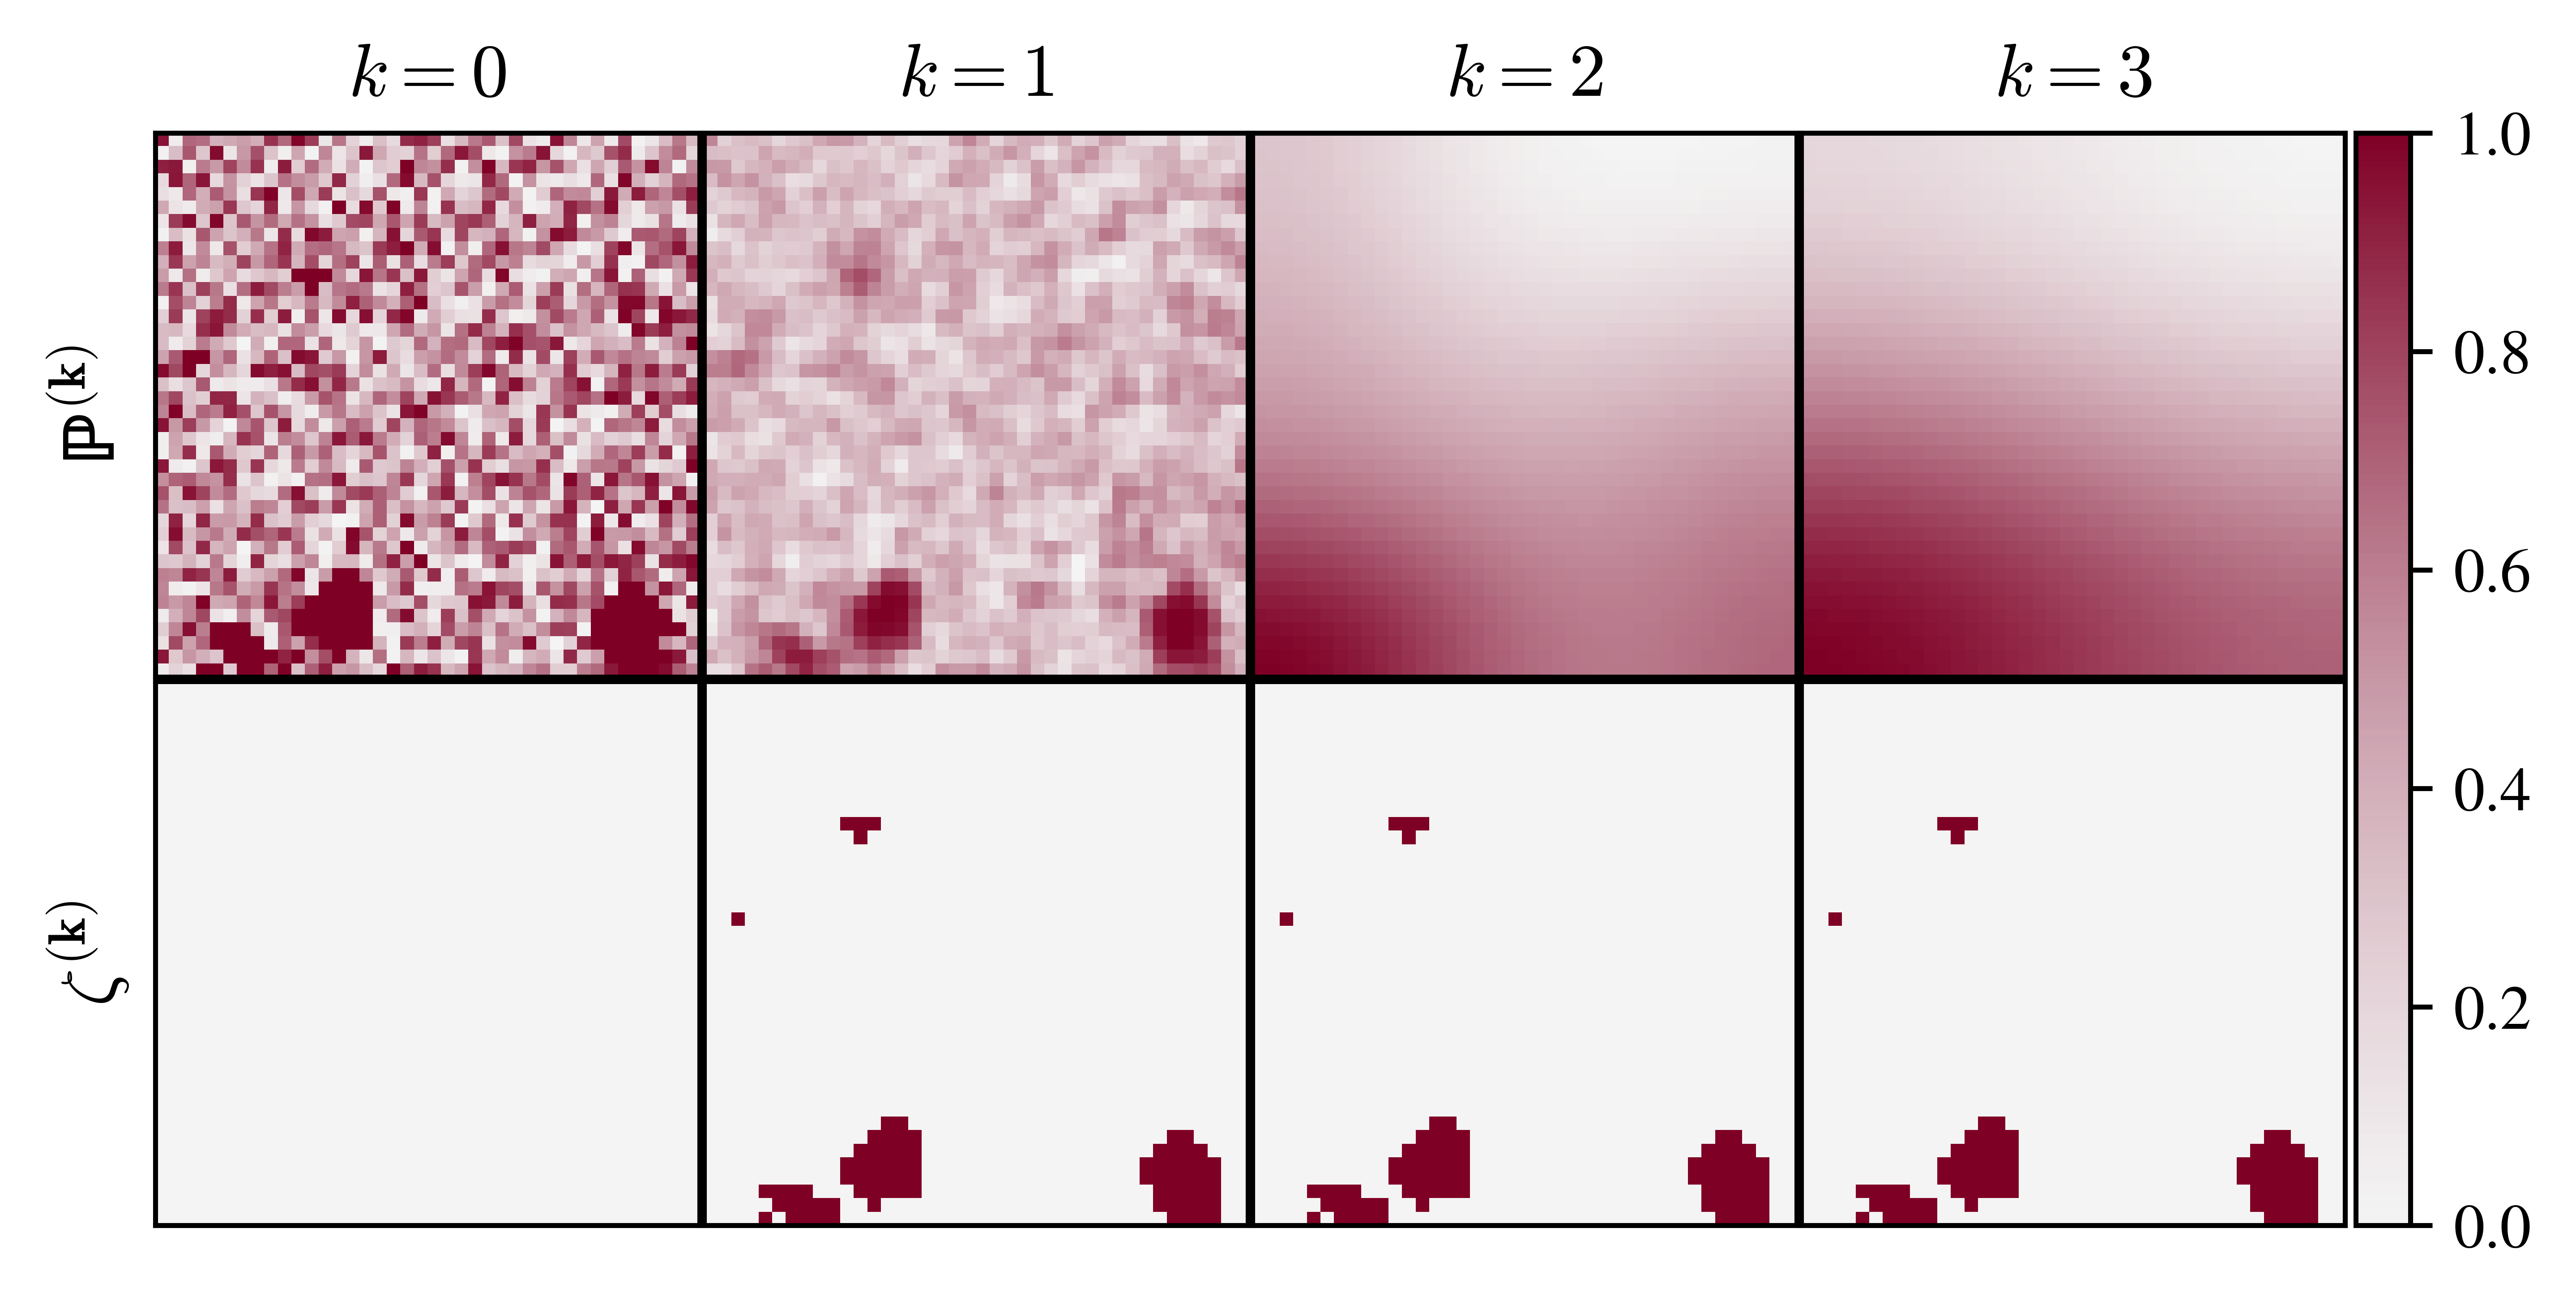
\includegraphics[width=0.65\textwidth]{Images/bfastEx3D.png}
\caption{Example in $z=20$ Plane of 3D Map for $p,q=0$}
\end{figure}
\end{frame}

\subsection{Performance Metrics}

%%%% 29
\begin{frame}{Performance Metrics}
\begin{itemize}
\item The performance of the bFAST algorithm was evaluated by comparing 
the final activation map with the true activation map using:
\begin{itemize}
\item \gls{ji}: Similarity between the two maps.
\item \gls{fpr}: Ratio of the voxels marked as activated that are not 
really active and the total number of inactive voxels.
\item \gls{poa}: Percentage of active voxels between both maps.
\end{itemize}
\item Performance was evaluated in each of the noise scenarios considered 
and an average value for the \gls{snr} and \gls{cnr} is also presented. 
\end{itemize}
\end{frame}

%%%% 30
\begin{frame}{Performance Metrics}
\begin{figure}
\centering
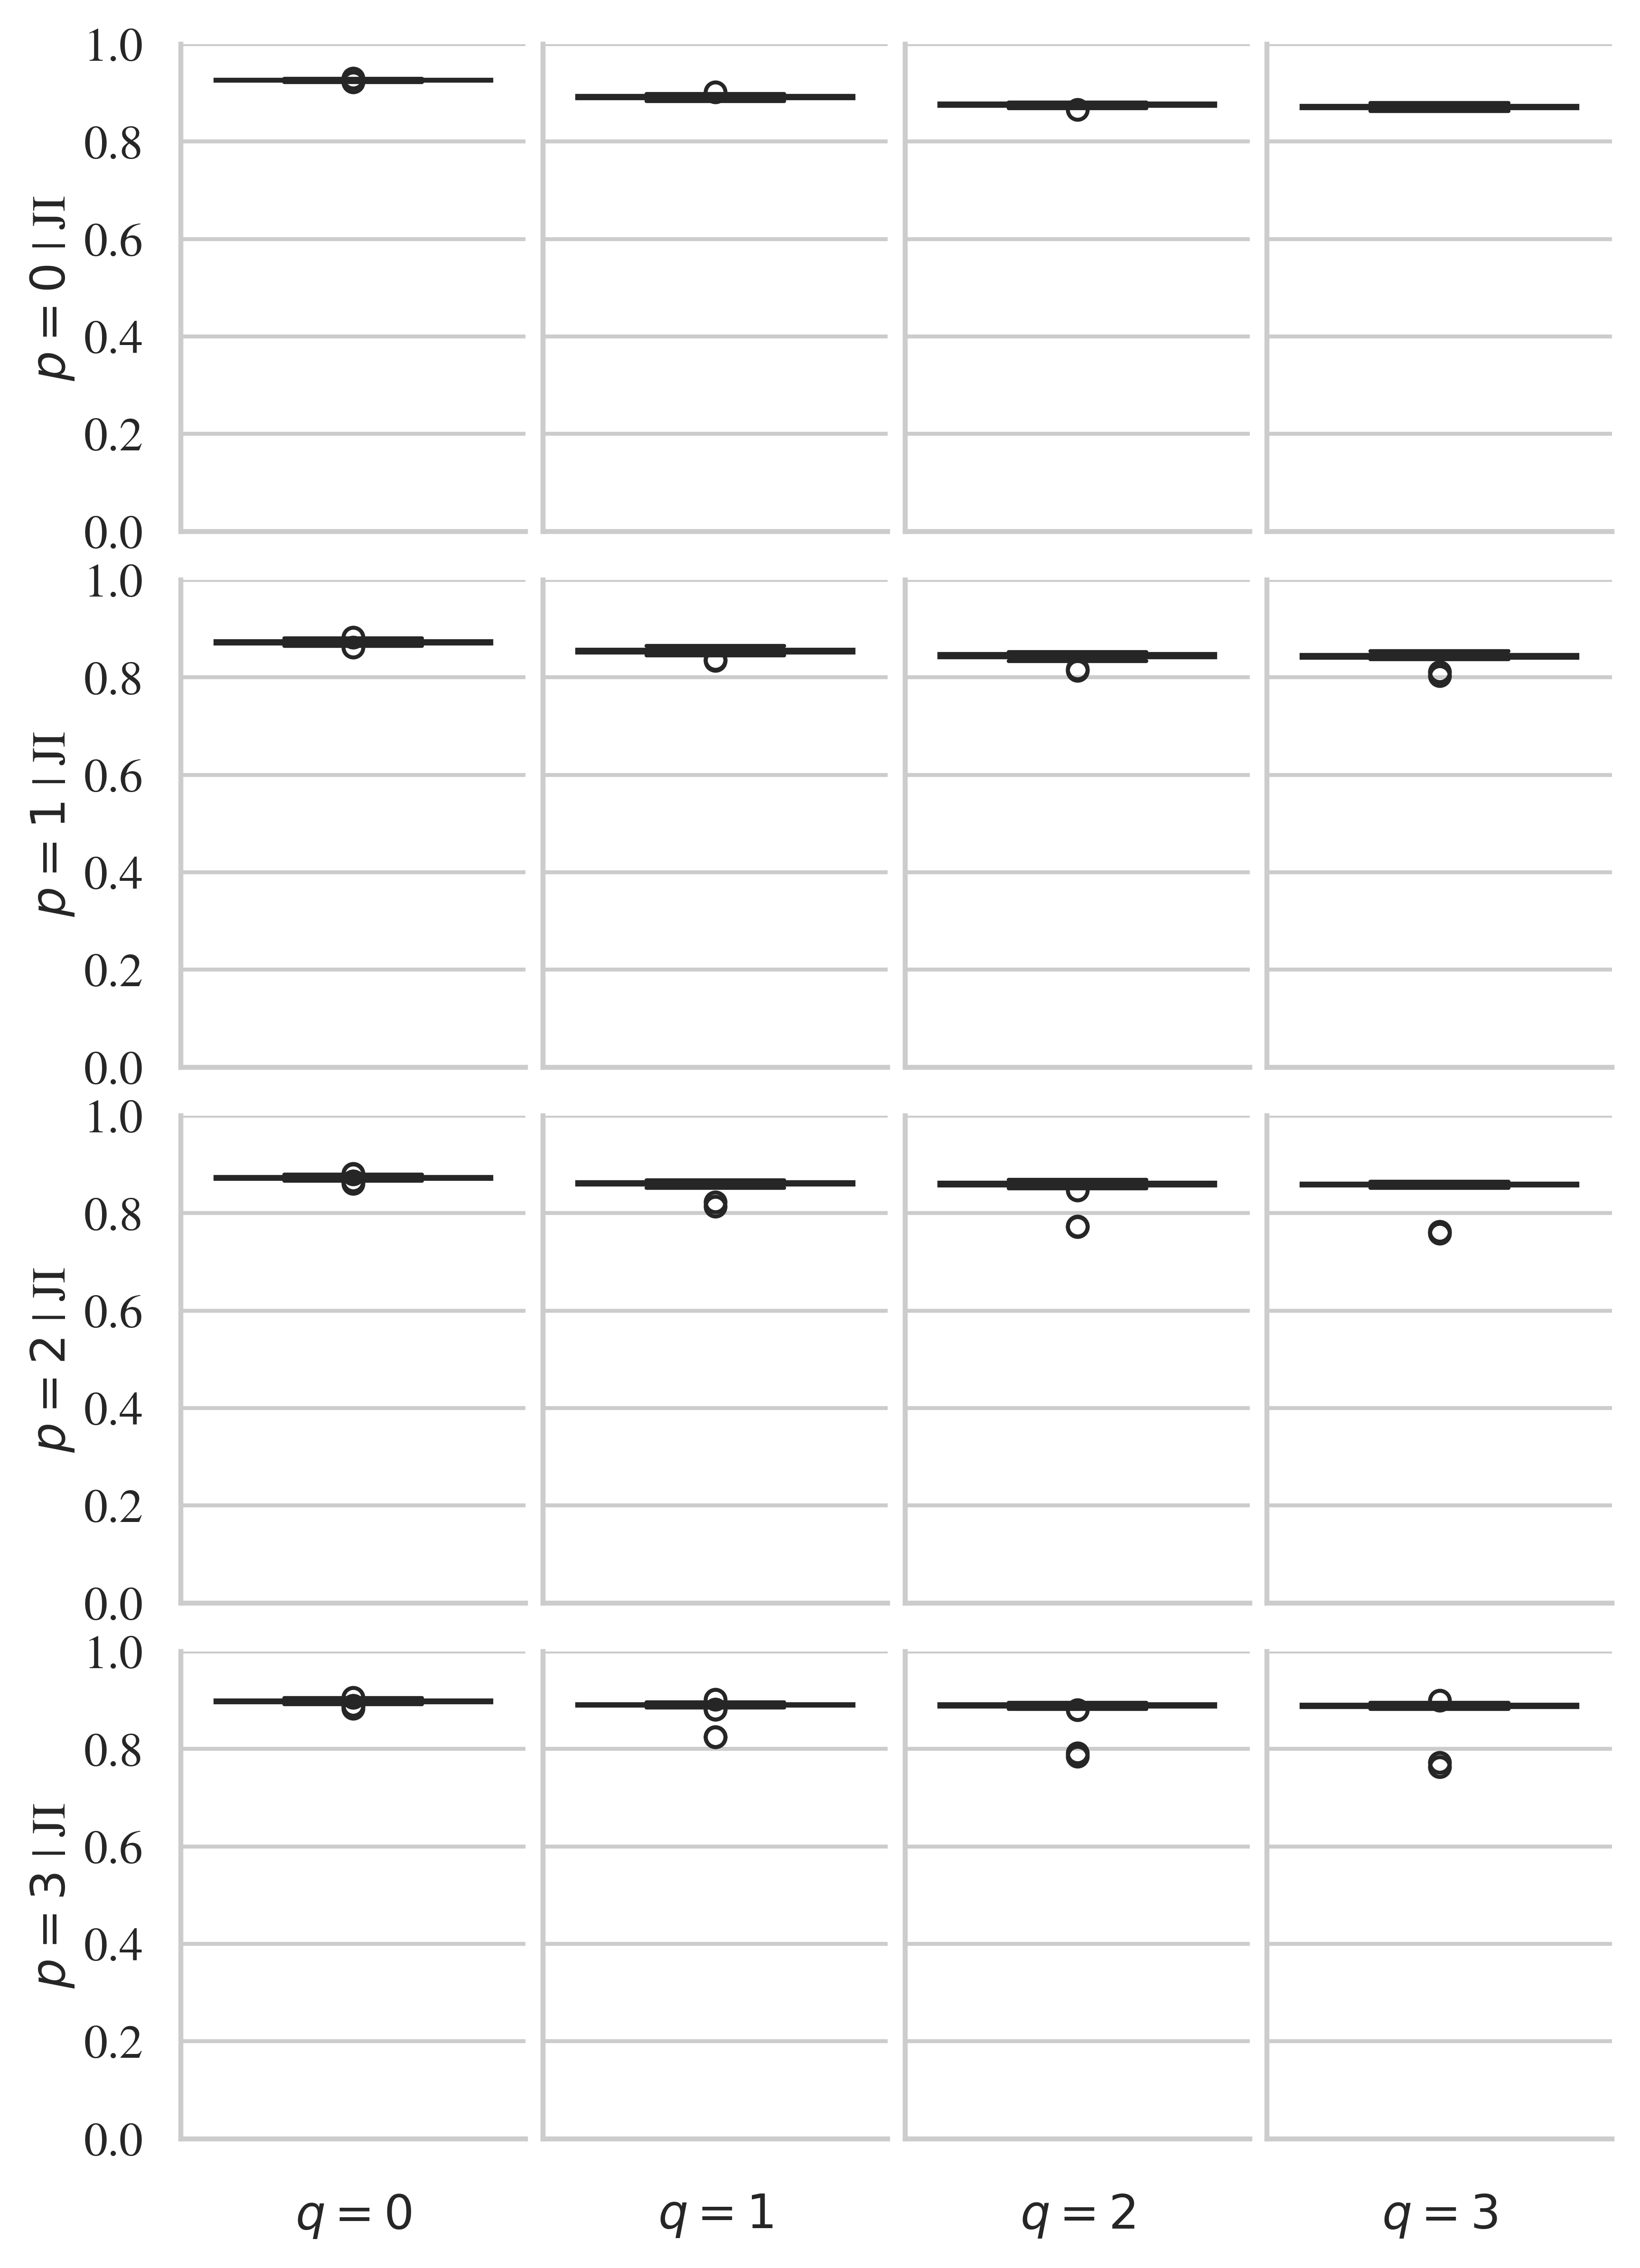
\includegraphics[width=0.4\textwidth]{Images/ji2D.png}
\caption{\acrlong{ji} in 2D Map}
\end{figure}
\end{frame}

%%%% 31
\begin{frame}{Performance Metrics}
\begin{figure}
\centering
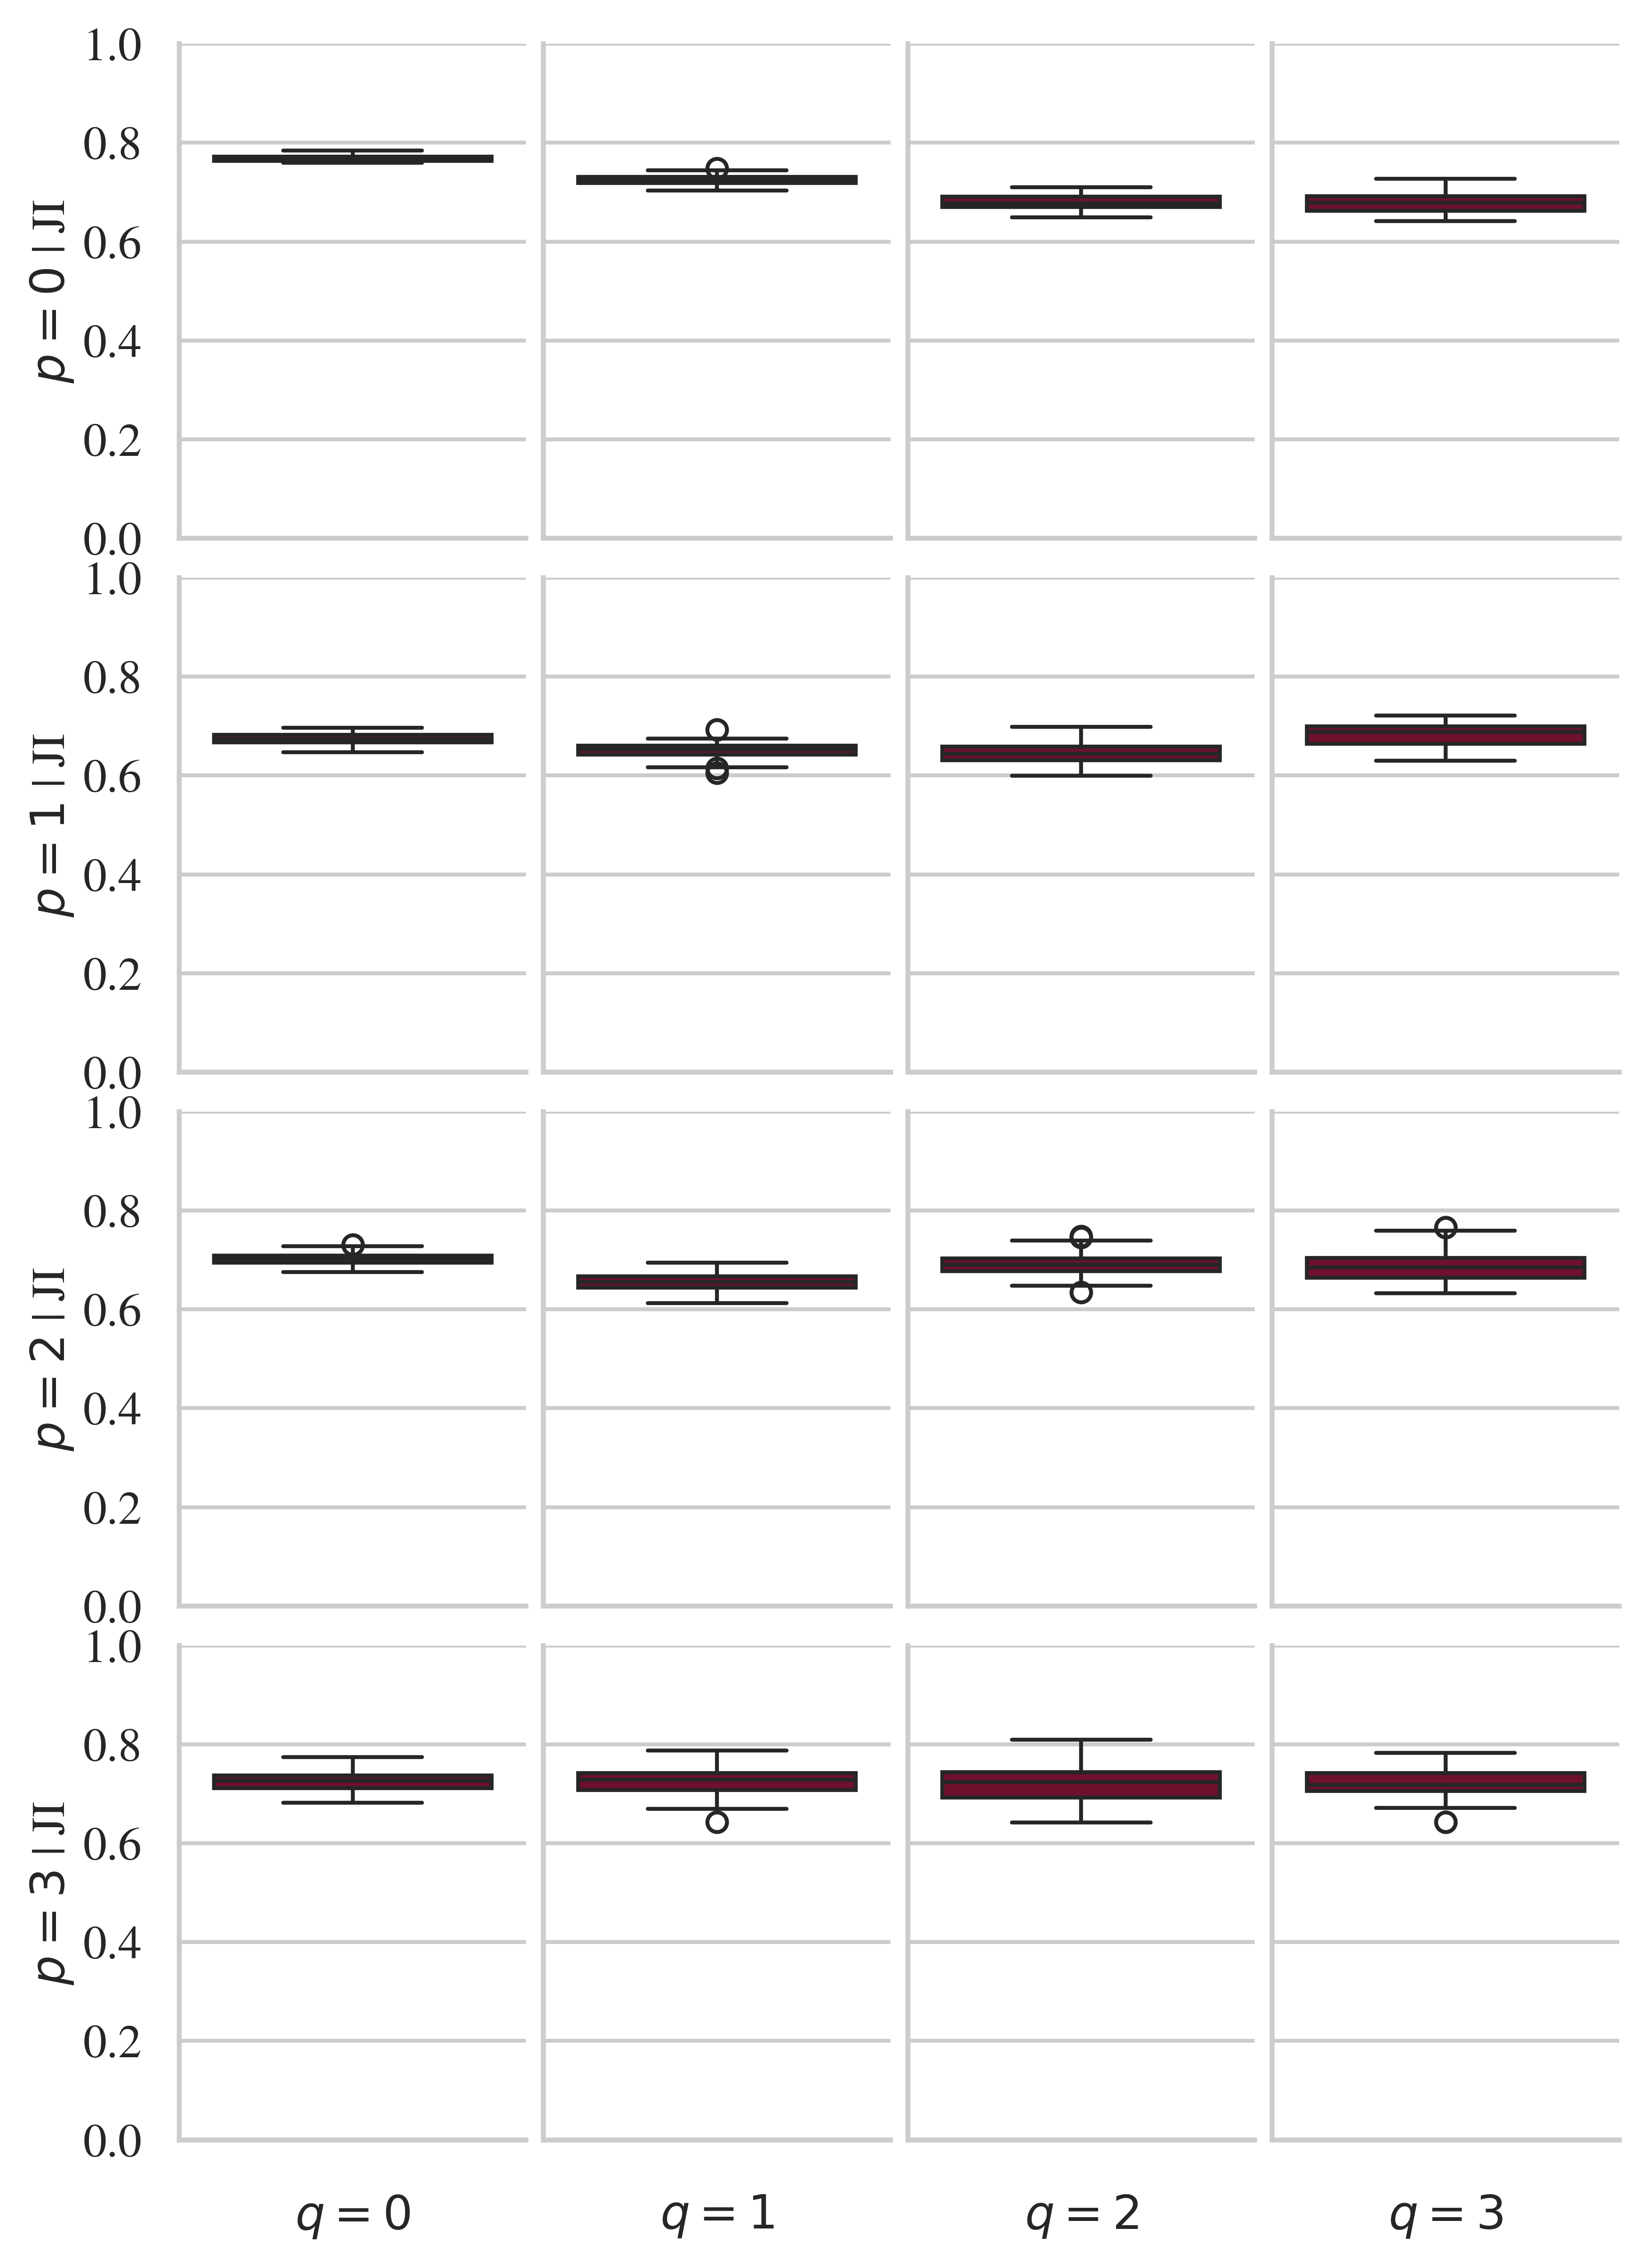
\includegraphics[width=0.4\textwidth]{Images/ji3D.png}
\caption{\acrlong{ji} in 3D Map}
\end{figure}
\end{frame}

\def\arraystretch{0.8}
\setlength{\tabcolsep}{4pt}
\abovecaptionskip=0pt
\belowcaptionskip=1pt 

%%%% 31
\begin{frame}{Performance Metrics}
\begin{table}
\centering
\caption{Performance Metrics Summary in 2D Case}
\begin{tabular}{ccccccc}
\hline
\textbf{P} & \textbf{Q} & \textbf{SNR} & \textbf{CNR} & \gls{ji} & \gls{fpr} & \gls{poa} \\ \hline
\multirow{4}{*}{0} & 0 & 4.0841 & 3.0344 & 0.9256 & 0.0078 & 19.663 \\
 & 1 & 3.6815 & 2.9342 & 0.8925 & 0.0180 & 20.515 \\
 & 2 & 3.5788 & 2.9035 & 0.8754 & 0.0227 & 20.858 \\
 & 3 & 3.5688 & 2.8960 & 0.8695 & 0.0244 & 20.995 \\ \hline
\multirow{4}{*}{1} & 0 & 3.5988 & 2.9042 & 0.8794 & 0.0222 & 20.870 \\
 & 1 & 2.7538 & 2.6993 & 0.8509 & 0.0299 & 21.398 \\
 & 2 & 2.5159 & 2.6191 & 0.8488 & 0.0308 & 21.475 \\
 & 3 & 2.4691 & 2.6007 & 0.8533 & 0.0292 & 21.350 \\ \hline
\multirow{4}{*}{2} & 0 & 2.9564 & 2.7050 & 0.8685 & 0.0240 & 20.908 \\
 & 1 & 2.1686 & 2.4761 & 0.8648 & 0.0267 & 21.228 \\
 & 2 & 1.8753 & 2.3861 & 0.8578 & 0.0284 & 21.333 \\
 & 3 & 1.8050 & 2.3646 & 0.8581 & 0.0283 & 21.313 \\ \hline
\multirow{4}{*}{3} & 0 & 2.5794 & 2.5607 & 0.8932 & 0.0174 & 20.445 \\
 & 1 & 1.8416 & 2.3420 & 0.8882 & 0.0185 & 20.513 \\
 & 2 & 1.5895 & 2.2576 & 0.8837 & 0.0200 & 20.638 \\
 & 3 & 1.5260 & 2.2323 & 0.8793 & 0.0213 & 20.740 \\ \hline
\end{tabular}
\end{table}
\end{frame}

%%%% 32
\begin{frame}{Performance Metrics}
\begin{table}
\centering
\caption{Performance Metrics Summary in 2D Case}
\begin{tabular}{ccccccc}
\hline
\textbf{P} & \textbf{Q} & \textbf{SNR} & \textbf{CNR} & \gls{ji} & \gls{fpr} & \gls{poa} \\ \hline
\multirow{4}{*}{0} & 0 & 4.0430 & 2.6156 & 0.7677 & 0.0046 & 3.8075 \\
 & 1 & 3.6401 & 2.5873 & 0.7249 & 0.0068 & 3.9950 \\
 & 2 & 3.5348 & 2.5699 & 0.6796 & 0.0086 & 4.0675 \\
 & 3 & 3.5233 & 2.5660 & 0.6767 & 0.0082 & 3.9950 \\ \hline
\multirow{4}{*}{1} & 0 & 3.5553 & 2.5687 & 0.6741 & 0.0092 & 4.1500 \\
 & 1 & 2.7134 & 2.4836 & 0.6468 & 0.0108 & 4.2650 \\
 & 2 & 2.4711 & 2.4406 & 0.6410 & 0.0116 & 4.3550 \\
 & 3 & 2.4303 & 2.4320 & 0.6757 & 0.0099 & 4.2625 \\ \hline
\multirow{4}{*}{2} & 0 & 2.9143 & 2.4583 & 0.6979 & 0.0083 & 4.1125 \\
 & 1 & 2.1205 & 2.3332 & 0.6566 & 0.0108 & 4.3100 \\
 & 2 & 1.8440 & 2.2791 & 0.6909 & 0.0079 & 4.0075 \\
 & 3 & 1.7735 & 2.2584 & 0.6859 & 0.0081 & 4.0300 \\ \hline
\multirow{4}{*}{3} & 0 & 2.5407 & 2.3554 & 0.7297 & 0.0065 & 3.9650 \\
 & 1 & 1.8073 & 2.2290 & 0.7194 & 0.0067 & 3.9525 \\
 & 2 & 1.5582 & 2.1729 & 0.7167 & 0.0074 & 4.0600 \\
 & 3 & 1.5004 & 2.1515 & 0.7092 & 0.0066 & 3.8925 \\ \hline
\end{tabular}
\end{table}
\end{frame}

\subsection{Real Case}

%%%% 33
\begin{frame}{bFAST in Real Data}
\begin{columns}

\column{0.35\linewidth}
\begin{figure}
\centering
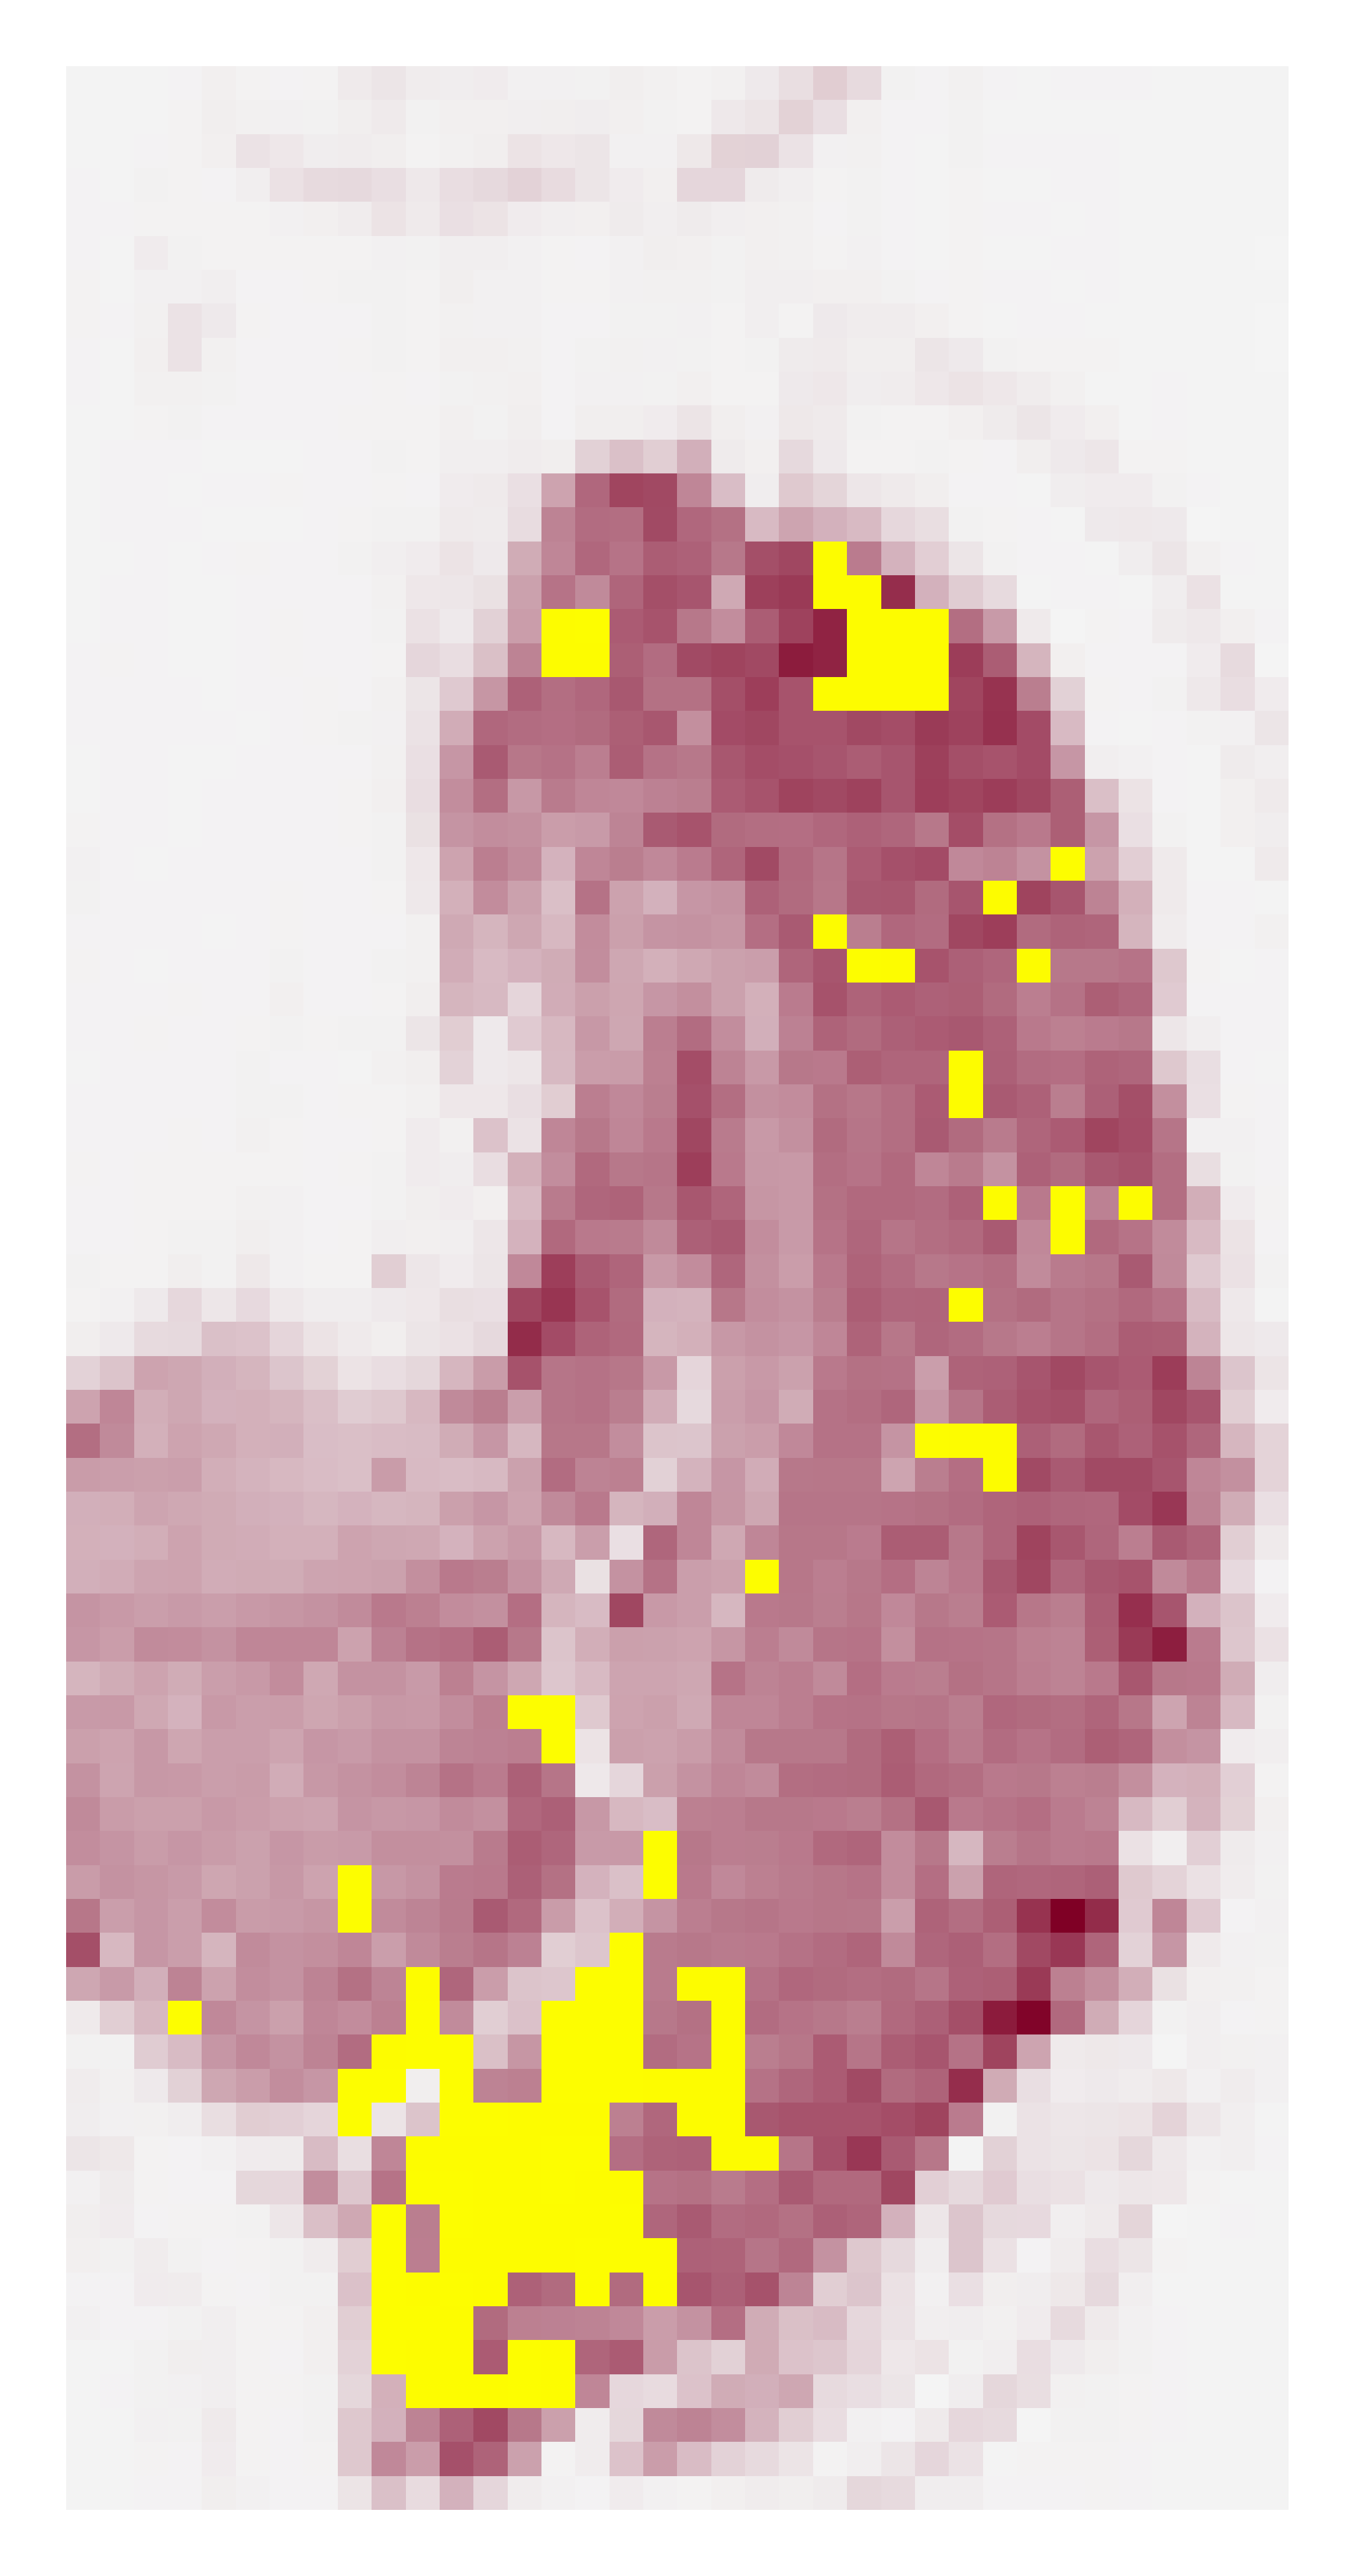
\includegraphics[angle=90,height=0.75in]{Images/realDataYZ.png}
\caption{$x=36$ Plane}
\end{figure}

\begin{figure}
\centering
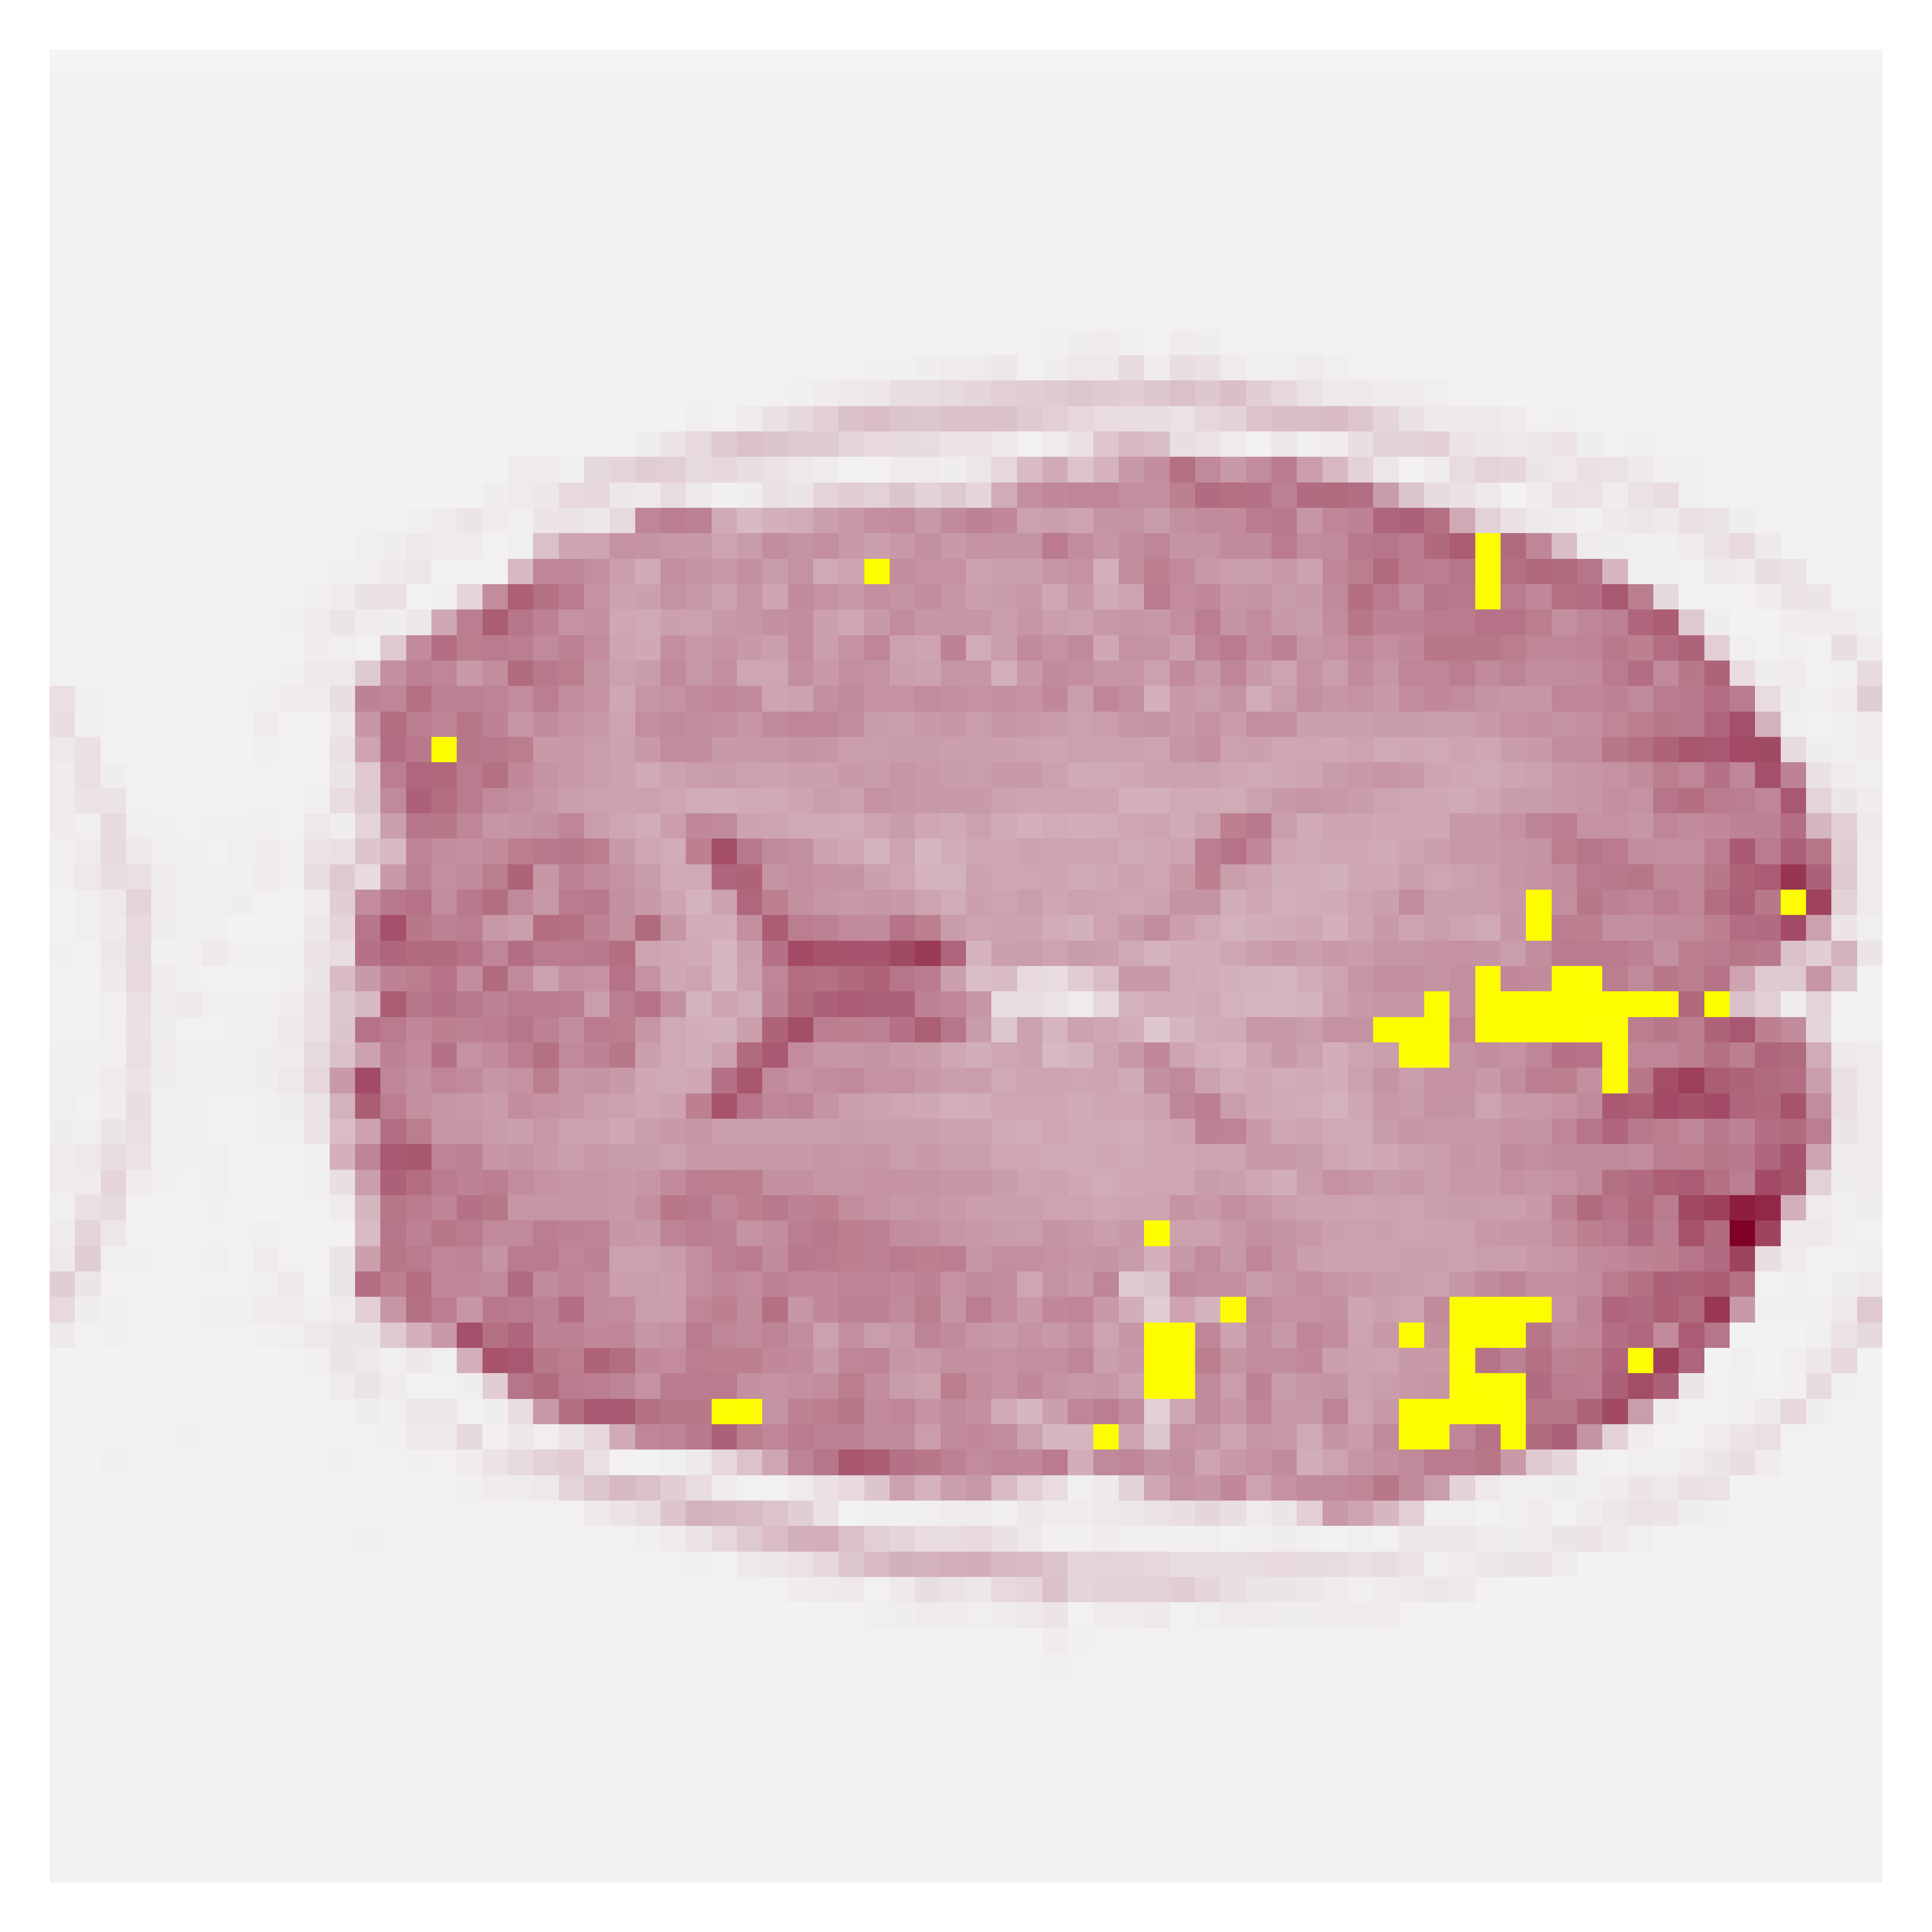
\includegraphics[height=0.75in]{Images/realDataXY.png}
\caption{$z=18$ Plane}
\end{figure}

\column{0.64\linewidth}
\begin{itemize}
\item Theory of Mind \gls{fmri} experiment
\item Gradient-echo echo-planar pulse sequence on a 3T Tim Trio MRI scanner
\item Stimulus is a false belief question
\item Data has dimensions $72\times72\times36$ of 2 mm isotropic voxels.
\item 40078 Voxels in the Region of Interest
\item bFAST identified 1766 active voxels (4.41 A\%)
\end{itemize}

\end{columns}
\end{frame}

\section{References}

%%%% 33-37
\begin{frame}[allowframebreaks]{References}
\bibliography{referencias}
\end{frame}

%%
\end{document}